\documentclass[a4paper,16pt]{jsarticle}

% 余白の設定
\setlength{\textwidth}{\fullwidth}
\setlength{\textheight}{40\baselineskip}
\addtolength{\textheight}{\topskip}
\setlength{\voffset}{-0.2in}
\setlength{\topmargin}{0pt}
\setlength{\headheight}{0pt}
\setlength{\headsep}{0pt}

% パッケージ
\usepackage[dvipdfmx]{hyperref,graphicx}		% 画像
\hypersetup{
	colorlinks=true, % リンクに色をつけない設定
	bookmarks=true, % 以下ブックマークに関する設定
	bookmarksnumbered=true,
	pdfborder={0 0 0},
	bookmarkstype=toc
}
\usepackage{amsmath, amssymb}		% ギリシャ文字
\usepackage{bm}				% 数式 \bm{a} aベクトル
\usepackage{comment}			% コメント
\usepackage{siunitx}			% SI単位
\usepackage{framed}			% 枠組み
\usepackage{braket}     % ブラケット記法

\newtheorem{theorem}{定理}
\newtheorem{proof}{証明}
\newcommand{\qed}{\qquad $\blacksquare$}

\begin{comment}
 複数行に渡るコメントの書き方
 \usepackage{comment}が必要。
\end{comment}

% section前に改ページ
\makeatletter
\def\section{\newpage\@startsection {section}{1}{\z@}{-3.5ex plus -1ex minus -.2ex}{2.3 ex plus .2ex}{\Large\bf}}
\makeatother

% 数式番号をいい感じに
\makeatletter
% \renewcommand{\theequation}{\arabic{chapter}-\arabic{section}-\arabic{equation}}
	\renewcommand{\theequation}{\arabic{section}-\arabic{equation}}
  \@addtoreset{equation}{section}
\makeatother

\title{量子力学}
\author{ゆきちゃん}
\date{\today}

\begin{document}
\maketitle

未来の自分が見返したときに、理解できるように書いています。
間違い等あれば、気軽に教えてください。

また、随時更新しています。書いている途中のもあります。

\tableofcontents

\newpage

% 
\section{memo}

波動関数の重ね合わせについての説明

エネルギー固有値

固有関数についての説明

井戸型ポテンシャルについて

摂動論がうまく適用できる範囲について


% 
\section{物理定数と次元解析}

\begin{table}[htb]

  \begin{tabular}{cc}

      質量 & $M$ \\
      時間 & $T$ \\
      長さ  & $L$ \\
  \end{tabular}
  \caption{}
  \label{}

\end{table}

\begin{table}[htb]

  \begin{tabular}{cc}

    真空中の高速 & $c$ \\
    電気素量     & $e$ \\


  \end{tabular}
  \caption{}
  \label{}

\end{table}


\begin{thebibliography}{99}
	\bibitem{} 猪木・河合、量子力学I、講談社サイエンティフィク、2017
	\bibitem{} 猪木・河合、量子力学II、講談社サイエンティフィク、2017
\end{thebibliography}

\section{時間に依存しないシュレディンガー方程式}
ポテンシャル$V$が時間に依存しない場合、変数分離を用いて解くことができる。

\begin{equation}
  i\hbar \dfrac{\partial \psi(x,t)}{\partial t} = - \dfrac{\hbar^2}{2m} \dfrac{\partial^2 \psi(x,t)}{\partial x^2} + V(x)\psi(x,t)
\end{equation}

今、波動関数$\psi(x,t)$が位置$x$と時間$t$についての関数$f(x)$、$g(t)$との積で書けるとする。

\begin{equation}
  \psi(x,t) = f(x)g(t)
\end{equation}

すると、

\begin{equation}
  i\hbar \dfrac{\partial f(x)g(t)}{\partial t} = - \dfrac{\hbar^2}{2m} \dfrac{\partial^2 f(x)g(t)}{\partial x^2} + V(x)f(x)g(t)
\end{equation}

左辺は$t$で、右辺は$x$での偏微分なので、

\begin{equation}
  i\hbar f(x)\dfrac{\partial g(t)}{\partial t} = - \dfrac{\hbar^2}{2m} g(t)\dfrac{\partial^2 f(x)}{\partial x^2} + V(x)f(x)g(t)
\end{equation}

ここで、両辺を$f(x)g(t)$で割ると、

\begin{equation}
  i\hbar \dfrac{1}{g(t)}\dfrac{\partial g(t)}{\partial t} = - \dfrac{\hbar^2}{2m} \dfrac{1}{f(x)}\dfrac{\partial^2 f(x)}{\partial x^2} + V(x)
\end{equation}

左辺は時間$t$に関して、右辺は位置$x$に関しての式になった。
つまり、両辺は$x$にも$t$にも依存しない定数である必要があり、この定数を$E$とする。

\begin{align}
  i\hbar \dfrac{1}{g(t)}\dfrac{d g(t)}{d t} = E \\
  - \dfrac{\hbar^2}{2m} \dfrac{1}{f(x)}\dfrac{d^2 f(x)}{d x^2} + V(x) = E
\end{align}

整理すると、

\begin{align}
  \label{eq.no.1}
  i\hbar \dfrac{d g(t)}{d t} = Eg(t) \\
  \label{eq.no.2}
  - \dfrac{\hbar^2}{2m} \dfrac{d^2 f(x)}{d x^2} = [ E-V(x) ]f(x)
\end{align}

(\ref{eq.no.1})、(\ref{eq.no.2})を解いていく。

(\ref{eq.no.1})は
\begin{align}
  i\hbar \dfrac{d g(t)}{d t} &= Eg(t) \\
  \dfrac{d g(t)}{d t} &= -i \dfrac{E}{\hbar} g(t)
\end{align}
より、
\begin{equation}
  \label{ans.no.1}
  \displaystyle g(t) = Ae^{-i \frac{E}{\hbar} t}
\end{equation}
と求まる。($A$は任意定数)

ここで、$\dfrac{E}{\hbar}$について考える。

(\ref{ans.no.1})は波であることから、$\dfrac{E}{\hbar}$は角速度$\omega$と分かる。

つまり、
\begin{equation}
  E = \hbar \omega
\end{equation}

これを変形すると、
\begin{align}
  E &= \hbar \omega \\
  &= \dfrac{h}{2\pi} 2\pi \nu \\
  &= h\nu
\end{align}

これは、粒子性と波動性を結ぶ大切な式であり、定数$E$はエネルギーと同じ次元を持つことが分かる。

次に、(\ref{eq.no.2})について考える。
\begin{equation*}
  \label{time_independent_schrodinger_eq}
  - \dfrac{\hbar^2}{2m} \dfrac{d^2 f(x)}{d x^2} = [ E-V(x) ]f(x)
\end{equation*}
これは、{\bf 時間に依存しないシュレディンガー方程式} と呼ばれる。

$V(x)$を具体的に決めることによって解くことができるかもしれない。

後にやる調和振動子ポテンシャルや井戸型ポテンシャルは解析的に解く事ができる。しかし、解析的に解く事ができるものばかりではない。
世の中、解析的に解けないものの方が多い。その場合は、コンピューターの力を使って数値的に解く。

また、変分法や摂動論を用いて解析的に精度良く求めることもできる。




\section{1次元シュレディンガー方程式の性質(その1)} \label{1dim_schrodinger_eq_propeties}
質量$m$の粒子が時間に依存しないポテンシャル$V(x)$で束縛されている時、この粒子の波動関数$\psi(x,t)$を決めることは、時間に依存しないシュレディンガー方程式
\begin{equation}
	- \dfrac{\hbar^2}{2m} \dfrac{d^2 \varphi(x)}{d x^2}= (E-V(x))\varphi(x)
\end{equation}
を解くことに帰着する。
この解の性質の$1$つに
{\bf $1$次元問題では、離散スペクトルの現れるエネルギー準位は縮退しない}
がある。

\begin{proof}
	エネルギー準位が縮退していると仮定する。
	つまり、異なる$2$つの波動関数$\varphi_1(x)$と$\varphi_2(x)$が同じエネルギー固有値$E$を持つ。この時、
	\begin{align}
		\dfrac{d^2 \varphi_1(x)}{dx^2} + \dfrac{2m}{\hbar^2}(E-V(x))\varphi_1(x) &= 0 \\
		\dfrac{d^2 \varphi_2(x)}{dx^2} + \dfrac{2m}{\hbar^2}(E-V(x))\varphi_2(x) &= 0
	\end{align}
	を満たす。
	それぞれ$\varphi_1$、$\varphi_2$で割ると、
	\begin{equation}
		\dfrac{1}{\varphi_1}\dfrac{d^2 \varphi_1}{dx^2} = \dfrac{2m}{\hbar^2}(E-V(x)) = \dfrac{1}{\varphi_2}\dfrac{d^2 \varphi_2}{dx^2}
	\end{equation}
	を得ることができる。
	これより、
	\begin{equation}
		\dfrac{1}{\varphi_1}\dfrac{d^2 \varphi_1}{dx^2} = \dfrac{1}{\varphi_2}\dfrac{d^2 \varphi_2}{dx^2}
	\end{equation}
	となり、両辺に$\varphi_1 \varphi_2$をかけると
	\begin{equation}
		\dfrac{d^2 \varphi_1}{dx^2}\varphi_2 = \dfrac{d^2 \varphi_2}{dx^2}\varphi_1
	\end{equation}
	左辺に寄せると、
	\begin{equation}
		\dfrac{d^2 \varphi_1}{dx^2}\varphi_2 - \dfrac{d^2 \varphi_2}{dx^2}\varphi_1 = 0
	\end{equation}
	これを変形すると、
	\begin{equation}
		\dfrac{d}{dx}\left[ \dfrac{d\varphi_1}{dx}\varphi_2 - \dfrac{d\varphi_2}{dx}\varphi_1\right] = 0
	\end{equation}
	となる。両辺を積分すると、
	\begin{equation}
		\dfrac{d\varphi_1}{dx}\varphi_2 - \dfrac{d\varphi_2}{dx}\varphi_1 = (定数)
	\end{equation}
	となる。
	今、粒子はポテンシャル$V$によって束縛されているので、無限遠で$\varphi_1 = \varphi_2 = 0$になる。
	つまり、定数は$0$でなければならない。
	従って、
	\begin{equation}
		\dfrac{1}{\varphi_1}\dfrac{d\varphi_1}{dx} = \dfrac{1}{\varphi_2}\dfrac{d \varphi_2}{dx}
	\end{equation}
	これを積分すると
	\begin{equation}
		\log\varphi_1 = \log\varphi_2 + 定数
	\end{equation}
	つまり、
	\begin{equation}
		\varphi_1 = \varphi_2 \times (定数)
	\end{equation}
	となり、$2$つの波動関数は本質的に同じものであることになる。
	これは波動関数が異なると仮定したことに矛盾する。
	よって、$1$次元問題では、離散スペクトルの現れるエネルギー準位は縮退しない。
	\qed
\end{proof}



\section{無限に深い1次元井戸型ポテンシャル}
無限に深い$1$次元井戸型ポテンシャルというものを考えてみよう。これはポテンシャル$V(x)$が
\begin{equation}
  V(x) =
  \begin{cases}
    0,       & (-a < x < a) \\
    \infty , & (x \leq -a , a \leq x)
  \end{cases}
\end{equation}
となっている。
$x \leq -a , a \leq x$でポテンシャルが無限大なので、この範囲で粒子は存在できない。
そのため、$-a < x < a$の範囲で時間に依存しないシュレディンガー方程式
\begin{equation}
  \label{time_independent_schrodinger_eq_in_well}
  - \dfrac{\hbar^2}{2m} \dfrac{d^2 \psi(x)}{d x^2} = E\psi(x)
\end{equation}
を解けばよい。
ここで、$x \leq -a , a \leq x$の範囲で粒子が存在できないことから、
境界条件
\begin{equation}
  \label{boundary_req}
  \psi(a) = \psi(-a) = 0
\end{equation}
を課すことになる。
(\ref{time_independent_schrodinger_eq_in_well})を変形して
\begin{equation}
  \dfrac{d^2 \psi(x)}{d x^2} = -\dfrac{2mE}{\hbar^2}\psi(x)
\end{equation}
ここで、
\begin{equation}
  \label{k_equiv}
  k \equiv \dfrac{\sqrt{2mE}}{\hbar}
\end{equation}
とおけば
\begin{equation}
  \dfrac{d^2 \psi(x)}{d x^2} = -k^2\psi(x)
\end{equation}
となり、この微分方程式を解けばよい。
一般解は
\begin{equation}
  \psi(x) = A\cos(kx) + B\sin(kx)
\end{equation}
となる。($A$、$B$は任意定数である。)

ここで、境界条件(\ref{boundary_req})より
\begin{align}
  A\cos(ka) + B\sin(ka) &= 0 \\
  A\cos(kx) - B\sin(kx) &= 0
\end{align}
これより、
\begin{align}
  A\cos(ka) &= 0 \\
  B\sin(ka) &= 0
\end{align}
が得られる。この条件を満たす解として$A=B=0$があるが、この時の波動関数$\psi(x)$は恒等的に$0$になるので、物理的に意味のない解になる。(つまり、粒子が存在しない状態になる。)

物理的に意味のある解を求めていこう。

$A = 0$の時、$B \neq 0$より
\begin{equation}
  \sin(ka) = 0
\end{equation}
つまり、
\begin{equation}
  ka = \dfrac{(n+1)\pi}{2}, \quad(n = 1, 3, 5, \ldots)
\end{equation}

$B = 0$の時、$A \neq 0$より
\begin{equation}
  \cos(ka) = 0
\end{equation}
つまり、
\begin{equation}
  ka = \dfrac{(n+1)\pi}{2}, \quad(n = 0, 2, 4, \ldots)
\end{equation}

従って、
\begin{equation}
  k = \dfrac{(n+1)\pi}{2a}, \quad(n = 0, 1, 2, \ldots)
\end{equation}
となる。
ここで、(\ref{k_equiv})より
\begin{equation}
  E = \dfrac{(n+1)^2\pi^2\hbar^2}{8ma^2}, \quad(n = 0,1,2,\ldots)
\end{equation}
と固有エネルギー$E$が求まる。

さて、固有状態の波動関数は
\begin{align}
  \psi(x) &= A\cos{\dfrac{(n+1)\pi}{2a}x}, \quad(n = 0, 2, 4, \ldots) \\
  \psi(x) &= B\sin{\dfrac{(n+1)\pi}{2a}x}, \quad(n = 1, 3, 5, \ldots)
\end{align}
と求まる。$n$が偶数の場合は、波動関数も偶関数であり、$n$が奇数の場合は、波動関数も奇関数であることが分かる。

定数$A$、$B$は波動関数の規格化定数である。
\begin{equation}
  1=\int_{-a}^{a} A^{2} \cos ^{2} k x \mathrm{d} x=A^{2} a, \quad
  1=\int_{-a}^{a} B^{2} \sin ^{2} k x \mathrm{d} x=B^{2} a
\end{equation}
より、
\begin{equation}
  A = B = \dfrac{1}{\sqrt{a}}
\end{equation}
と求めることができる。



\section{1次元調和振動子ポテンシャル}
$x$軸上で原点からの距離に比例する引力を受けて単振動する粒子について考える。
この時の粒子のポテンシャルエネルギーは角振動数$\omega$を用いて、$V(x) = \dfrac{1}{2}m\omega x^2$とかける。
よって、ポテンシャルは位置にのみ依存するので、時間に依存しないシュレディンガー方程式を用いて

\begin{equation}
	\label{harmony_schrodinger_eq}
	E\psi(x) = - \dfrac{\hbar^2}{2m} \dfrac{d^2 \psi(x)}{d x^2} + \dfrac{1}{2}m\omega x^2\psi(x)
\end{equation}

となる。このままでも解くことができるが、式を簡単にして見通しをよくしたい。
そのためには、
\begin{align}
		\label{xi}
		\xi &= \sqrt{\dfrac{m\omega}{\hbar}}x \\
		\label{eps}
		\epsilon &= \dfrac{2E}{\hbar\omega}
\end{align}
という、無次元の変数$\xi$、$\epsilon$を導入する。

(\ref{harmony_schrodinger_eq})の両辺に$\dfrac{2}{\hbar\omega}$をかけると、

\begin{equation}
	\dfrac{2E}{\hbar\omega}\psi(x) = - \dfrac{\hbar}{m\omega} \dfrac{d^2 \psi(x)}{d x^2} + \dfrac{m\omega}{\hbar} x^2\psi(x)
\end{equation}

変形して、
\begin{equation}
	\dfrac{2E}{\hbar\omega}\psi(x) = - \dfrac{d^2 \psi(x)}{d \dfrac{m\omega}{\hbar} x^2} + \dfrac{m\omega}{\hbar} x^2\psi(x)
\end{equation}
(\ref{xi})、(\ref{eps})より、
\begin{equation}
	\epsilon\psi(\xi) = - \dfrac{d^2 \psi(\xi)}{d \xi^2} + \xi^2\psi(\xi)
\end{equation}
よって、
\begin{equation}
	\label{harmony_DE}
	\dfrac{d^2 \psi(\xi)}{d \xi^2} + (\epsilon - \xi^2)\psi(\xi) = 0
\end{equation}
となる。
この微分方程式を解けば良いのだが、これが難しい。
上手い具合に近似できないか考えてみる。
$\xi \to \pm \infty$では$\epsilon$は$\xi$に比べて小さいので無視できそうだ。
すると、
\begin{equation}
	\dfrac{d^2 \psi(\xi)}{d \xi^2}  - \xi^2\psi(\xi) = 0
\end{equation}
これは簡単に解く事ができて、
\begin{equation}
	\psi(\xi) = He^{\pm \frac{\xi^2}{2}}
\end{equation}
となる。($H$は任意定数)
$\xi \to \pm\infty$の極限では波動関数$\psi$は収束しなければいけない。
そのため、指数部分の符号は負である必要がある。よって、
\begin{equation}
	\psi(\xi) = He^{-\frac{\xi^2}{2}}
\end{equation}
これは、$\xi \to \pm \infty$の極限を仮定した解であることに注意しなければならない。
実際に、これを(\ref{harmony_DE})に戻してみると、当然解になっていない事が確認できる。
この解を元に$\xi \to \pm \infty$の極限以外でも成立するような解を探す。
では、どうすれば良いのかというと、定数$H$が実は$\xi$の関数$H(\xi)$であると仮定する上手く行く。

今、
\begin{equation}
	\psi(\xi) = H(\xi)e^{-\frac{\xi^2}{2}}
\end{equation}

これを(\ref{harmony_DE})に戻す。
積の微分であることに注意すると、
\begin{equation}
	\dfrac{d\psi(\xi)}{d\xi} = e^{-\frac{\xi^2}{2}}\dfrac{dH(\xi)}{d\xi} - \xi H(\xi)e^{-\frac{\xi^2}{2}}
\end{equation}
\begin{equation}
	\dfrac{d^2\psi(\xi)}{d\xi^2} = e^{-\frac{\xi^2}{2}}\dfrac{d^2 H(\xi)}{d\xi^2} -2\xi e^{-\frac{\xi^2}{2}}\dfrac{dH(\xi)}{d\xi}
	 															+ (\xi^2 - 1)H(\xi)e^{-\frac{\xi^2}{2}}
\end{equation}

なので、(\ref{harmony_DE})に戻すと、

\begin{equation}
	\label{H_DE}
	\left[\dfrac{d^2}{d\xi^2} -2\xi\dfrac{d}{d\xi} + (\epsilon -1)\right]H(\xi) = 0
\end{equation}

この微分方程式を解くことになる。
これを解くために、$H(\xi)$が級数展開できると仮定する。
\begin{equation}
	H(\xi) = \sum_{k=0}^{\infty}a_k \xi^k
\end{equation}
この$a_k$を求める事ができれば、$H(\xi)$が決まるので、微分方程式が解けたことになる。
微分すると、
\begin{equation}
	\dfrac{d H(\xi)}{d\xi} = \sum_{k=1}^{\infty}a_k k\xi^{k-1} = \sum_{k=0}^{\infty}a_k k\xi^k
\end{equation}
\begin{equation}
	\dfrac{d^2 H(\xi)}{d\xi} = \sum_{k=2}^{\infty}a_k k(k-1)\xi^{k-2} = \sum_{k=0}^{\infty}a_{k+2} (k+2)(k+1)\xi^k
\end{equation}
よって、(\ref{H_DE})に戻すと、
\begin{equation}
	\sum_{k=0}^{\infty} \left[ (k+2)(k+1)a_{k+2} - (2k - \epsilon + 1)a_k  \right] \xi^k = 0
\end{equation}
これより、
\begin{equation}
	(k+2)(k+1)a_{k+2} = (2k - \epsilon + 1)a_k
\end{equation}
という事がわかるので、
\begin{equation}
	\label{recurrence_relation_1}
	a_{k+2} = \dfrac{(2k - \epsilon + 1)}{(k+2)(k+1)}a_k
\end{equation}
となり、
\begin{itemize}
	\item $a_0$が決まれば、偶数次の項
	\item $a_1$が決まれば、奇数次の項
\end{itemize}
が決まることになる。

$H(\xi)$は無限級数である。その為、発散するのか収束するのか気になる。

$k \to \infty$の時、$a_{k+2} \approx \dfrac{2}{k}a_k$と近似できる。
$k = 2n$とすると、$a_{2(n+1)} \approx \dfrac{1}{n}a_{2n}$となる。
なので、
\begin{equation}
	H(\xi) \approx \sum_{n}\dfrac{1}{n!}\xi^{2n} \approx e^{\xi^2}
\end{equation}
すると、
\begin{equation}
	\psi(\xi) = H(\xi)e^{-\frac{\xi^2}{2}} \approx e^{\frac{\xi^2}{2}}
\end{equation}
となり、$\xi \to \infty$で発散してしまう。
$H(\xi)$が無限級であるために発散してしまうのだ。
なので、収束させるために$H(\xi)$が有限個の項で終わるような条件を付けてやれば良い。
(\ref{recurrence_relation_1})より、
\begin{equation}
	\label{eps_requirement}
	\epsilon = 2n + 1
\end{equation}
とすれば、第$n$項は存在するが、第$n+2$項から$0$になる。
第$n+1$項も$0$であって欲しいので、
\begin{itemize}
	\item $n$が偶数 $\Rightarrow a_1 = 0$
	\item $n$が奇数 $\Rightarrow a_0 = 0$
\end{itemize}
という条件を付けて、$n$が偶数の時は奇数次の項が、$n$が奇数の時は偶数次の項が$0$になるようにしてしまえば良い。

$n$によって、$H(\xi)$が変わるので、$H_n(\xi)$と書くようにする。

いくつか計算してみると、
$$
\begin{aligned} H_{0}(\xi) &=a_{0} \\ H_{1}(\xi) &=a_{1} \xi \\ H_{2}(\xi) &=a_{0}\left(1-\frac{4}{1 \cdot 2} \xi^{2}\right) \\ H_{3}(\xi) &=a_{1}\left(\xi-\frac{4}{2 \cdot 3} \xi^{3}\right) \\ H_{4}(\xi) &=a_{0}\left(1-\frac{8}{1 \cdot 2} \xi^{2}+\frac{8}{1 \cdot 2} \frac{4}{3 \cdot 4} \xi^{5}\right) \\ & \vdots
\end{aligned}
$$

これの$H_n(\xi)$を{\bf エルミート(Hermite)多項式}と呼ぶ。

一般的に、エルミート多項式は
\begin{equation}
	H_{n}(\xi)=(-1)^{n} e^{\xi^{2}} \frac{\mathrm{d}^{n}}{\mathrm{d} \xi^{n}} e^{-\xi^{2}}
\end{equation}
と書ける。
いくつか計算してみると、
\begin{equation}
\begin{aligned}
	H_{0}(\xi) &= 1 \\
	H_{1}(\xi) &= 2 \xi \\
	H_{2}(\xi) &= 4 \xi^{2}-2 \\
	H_{3}(\xi) &= 8 \xi^{3}-12 \xi \\
						 & \vdots \end{aligned}
\end{equation}

$a_0$と$a_1$が$n$によって違うが、微分方程式(\ref{H_DE})を満たすので気にしなくて良い。

以上のことより、
\begin{equation}
	\label{harmony_psi}
	\psi_n(\xi) = H_n(\xi)e^{-\frac{\xi^2}{2}}
\end{equation}
と、(\ref{harmony_schrodinger_eq})を解く事ができた。

ここで、(\ref{eps})と、(\ref{eps_requirement})を思い出してみよう。
これらより、
\begin{equation}
	E_n = \hbar\omega(n+\frac{1}{2})
\end{equation}
$n$は$0$を含む正の整数である。(エルミート多項式を定義するため)

$n = 0$の時、$E_0 = \frac{1}{2}\hbar\omega$である。
つまり、調和振動子ポテンシャルでは、粒子の持つエネルギーは$0$にはならない。

エネルギーが$0$の状態は粒子が止まっていることを表す。
つまり、運動エネルギーが$0$であり、ポテンシャルエネルギーも$0$である。
ということは、運動量は$0$で、粒子は原点にあるという事がわかる。
位置と運動量が同時に確定してしまい、不確定性原理に反してしまう。
だから、エネルギーは$0$にはならない。

エネルギーが$0$にならないということは、このポテンシャルの中で粒子は振動をし続ける事になる。
位置と運動量を同時に確定させないためだ。
この、$n=0$の時の振動を{\bf 零点振動}と呼び、この時のエネルギー$E_0$のことを{\bf 零点エネルギー}と呼ぶ。

さて、(\ref{harmony_psi})より、波動関数を求める事ができたので、実際に波動関数の形を見てみよう。
固有エネルギー$En$と対応する波動関数$\psi_n$を$n=11$までplotしたものだ。
波動関数は固有エネルギー分を平行移動してあり、規格化されている。
\begin{figure}[htb]
	\begin{center}
		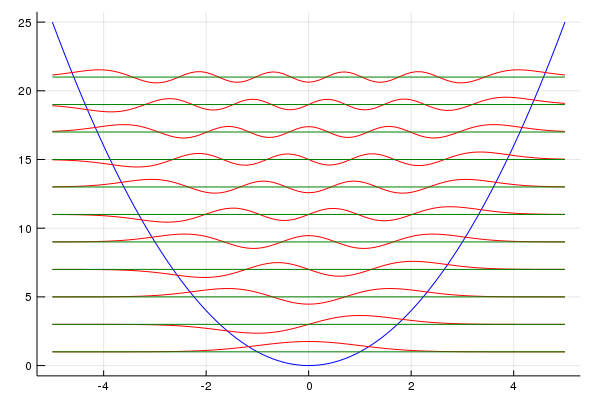
\includegraphics[height=6cm]{../fig/harmony.png}
		\caption{調和振動子ポテンシャルと波動関数($n=11$まで)}
		\label{}
	\end{center}
\end{figure}

量子的なミクロな世界にバネは存在しない。しかし、粒子が移動しようとしても元の位置に戻すような力、復元力が働くような状況を条件によっては作り出せるわけだ。
そのような復元力を級数展開して
\begin{equation}
	V(x) = a_0 + a_1 x + a_2 x^2 + a_3 x^3 + a_4 x^4 + \cdots
\end{equation}
と書けるとしよう。
$x$がとても小さい時、$3$次以降の項は$2$次の項に比べてほとんど無視できる程に小さい。
そして、$0$次と$1$次の項は$V(x) = a_2 x^2$を平行移動させる意味しかない。結局、考えるのは$2$次の項だけで十分であり、調和振動子ポテンシャルと同じ形になる。
なので、復元力によって粒子が振動しているような状況はこの調和振動子と同じ様な振る舞いになる。そのため、この調和振動子型ポテンシャルはとても重要なのだ。また、場合によっては$3$次や$4$次といった、高次の項を無視せずにもっと精密に解く場合はどうすれば良いのだろうか?それは摂動論を学ぶ必要がある。



\section{調和振動子ポテンシャルと昇降演算子}
再び調和振動子ポテンシャルだ。
今回は、昇降演算子というものを用いて調和振動子ポテンシャルのシュレディンガー方程式
\begin{equation}
  \label{harmony_schrodinger_eq}
  E\psi(x) = - \dfrac{\hbar^2}{2m} \dfrac{d^2 \psi(x)}{d x^2} + \dfrac{1}{2}m\omega x^2\psi(x)
\end{equation}
を解く。それから、求めた波動関数の規格化もする。
以前と同様に無次元の量

\begin{align}
  \label{y}
  y &= \sqrt{\dfrac{m\omega}{\hbar}}x \\
  \label{eps}
  \epsilon &= \dfrac{2E}{\hbar\omega}
\end{align}
を導入して、
\begin{equation}
  \label{harmony_DE}
  \left( -\dfrac{d^2}{d y^2} + y^2 \right) \psi(y) = \epsilon\psi(y)
\end{equation}
ここで、{\bf 昇降演算子}
\begin{align}
  \label{U}
  U &= \dfrac{d}{dy} - y \\
  \label{D}
  D &= \dfrac{d}{dy} + y
\end{align}
を定義する。

この演算子$U、D$の性質を見ていこう。
任意の関数$f$に対して、積$UD$は
\begin{align}
  UDf &= \left( \dfrac{d}{dy} - y \right)\left( \dfrac{d}{dy} + y \right)f \\
  &= \dfrac{d^2f}{dy^2} + \dfrac{d}{dy}(yf) - y\dfrac{df}{dy} - y^2 f \\
  &= \dfrac{d^2f}{dy^2} + f +  y\dfrac{df}{dy} - y\dfrac{df}{dy} - y^2 f \\
  &= \dfrac{d^2f}{dy^2} -y^2 f + f \\
  &= \left( \dfrac{dy^2}{d^2} -y^2 + 1\right)f
\end{align}
ハミルトニアン$H = -\dfrac{d^2}{d^2} + y^2$を用いて
\begin{equation}
  \label{UD}
  UD = -H + 1
\end{equation}
同様に、積$DU$は
\begin{equation}
  \label{DU}
  DU = -H - 1
\end{equation}
となる。つまり、演算子$U、D$は非可換である。なので、演算の順序には注意しなければならない。

次に、(\ref{UD})に左から$D$を作用させる。
\begin{equation}
  DUD = D(-H+1) = -DH + D
\end{equation}
(\ref{DU})より、
\begin{equation}
  (-H-1)D = -HD-D = -DH + D
\end{equation}
よって、
\begin{equation}
  \label{DH}
  DH = HD + 2D
\end{equation}
シュレディンガー方程式(\ref{harmony_DE})をハミルトニアン$H$を用いて、
\begin{equation}
  \label{Hpsi}
  H\psi = \epsilon\psi
\end{equation}
これに、左から$D$を作用させると
\begin{equation}
  DH\psi = D\epsilon\psi
  = \epsilon D \psi
\end{equation}
(\ref{DH})より、
\begin{equation}
  (HD + 2D)\psi = \epsilon D \psi
\end{equation}
よって、
\begin{equation}
  H(D\psi) = (\epsilon-2)(D\psi)
\end{equation}
これは、$D\psi$という波動関数が同じハミルトニアン$H$に対して、$\epsilon-2$という$2$だけ小さい固有値を持つ固有関数であることを示している。

同様の操作をすると
\begin{equation}
  H(D^2\psi) = (\epsilon-4)(D^2\psi)
\end{equation}
になることが確認できる。
一般的に、
\begin{equation}
  H(D^n\psi) = (\epsilon-2n)(D^n\psi)
\end{equation}
同様に、
\begin{equation}
  H(U^n\psi) = (\epsilon+2n)(U^n\psi)
\end{equation}
以上のことより、
$D$を作用させると、現在の固有値より$2$だけ小さい固有値と対応する固有関数$D\psi$を、
$U$を作用させると、現在の固有値より$2$だけ大きい固有値と対応する固有関数$U\psi$を、
求める事ができる。
これが昇降演算子の性質である。

この性質を用いて、調和振動子ポテンシャルのエネルギー固有値と対応する固有関数(波動関数)を求めていく。

基底状態のエネルギーを$\epsilon_0$、この時の固有関数を$\psi_0$とすると、
\begin{equation}
  H\psi_0 = \epsilon_0\psi_0
\end{equation}
これに左から$D$を作用させて整理すると、
\begin{equation}
  H(D\psi_0) = (\epsilon_0 - 2)(D\psi_0)
\end{equation}
となるが、$\epsilon_0$は基底状態のエネルギーなので、これ以上小さくなることはない。
つまり、
\begin{equation}
  \label{D}
  D\psi_0 = 0
\end{equation}
である必要がある。また、これに左から$U$を作用させて(\ref{UD})を使うと
\begin{equation}
  UD\psi_0 = (-H+1)\psi_0 = 0
\end{equation}
つまり、
\begin{equation}
  H\psi_0 = \psi_0
\end{equation}
このことから、基底状態のエネルギー$\epsilon_0 = 1$とわかる。
また、$U$を作用させるとエネルギーが$2$増えるので、$\epsilon_1 = 1+2$、$\epsilon_2 = 1+4$、$\ldots$となるので
\begin{equation}
  \label{eps_requirement2}
  \epsilon_n = 2n + 1
\end{equation}
となる事がわかる。

基底状態のエネルギーが求まったので、対応する固有関数を求める。
微分方程式(\ref{D})
\begin{equation}
  D\psi_0 = \left( \dfrac{d}{dy} +1 \right)\psi_0 = 0
\end{equation}
を解けば良い。
これは変数分離を用いると簡単に解く事ができて、解は
\begin{equation}
  \psi_0 = Ce^{\frac{-y^2}{2}}
\end{equation}
となる。($C$は任意定数)

さて、基底状態の波動関数が求まったので、規格化しよう。
\begin{equation}
  \int_{-\infty}^\infty |\psi_0|^2 dx = |C|^2 \int_{-\infty}^\infty e^{\frac{-y^2}{2}} dx = 1
\end{equation}
より、$C$を決定すれば良い。
(\ref{y})より
\begin{equation}
  |C|^2 \int_{-\infty}^\infty e^{\frac{-y^2}{2}} dx = |C|^2 \int_{-\infty}^\infty e^{\frac{-y^2}{2}} \sqrt{\dfrac{\hbar}{m\omega}}dy
  = |C|^2\sqrt{\dfrac{\hbar}{m\omega}}\sqrt{\pi} = 1
\end{equation}
よって、
\begin{equation}
  C = \left( \dfrac{m\omega}{\hbar\pi} \right)^\frac{1}{4}
\end{equation}
従って、規格化された基底状態の波動関数は、
\begin{equation}
  \psi_0(y) = \left( \dfrac{m\omega}{\hbar\pi} \right)^\frac{1}{4}e^{\frac{-y^2}{2}}
\end{equation}

励起状態の波動関数は$U$を作用させてやれば求まる。
実際に、
\begin{align}
  \psi_1 &= U\psi_0 \\
  &= \left( \dfrac{m\omega}{\hbar\pi} \right)^\frac{1}{4}\left(\dfrac{d}{dy} - y\right)e^{\frac{-y^2}{2}} \\
  &= \left( \dfrac{m\omega}{\hbar\pi} \right)^\frac{1}{4}\left( -2ye^{\frac{-y^2}{2}} \right)
\end{align}
\begin{align}
  \psi_2 &= U\psi_1 \\
  &= \left( \dfrac{m\omega}{\hbar\pi} \right)^\frac{1}{4}\left(\dfrac{d}{dy} - y\right)\left( -2ye^{\frac{-y^2}{2}} \right) \\
  &= \left( \dfrac{m\omega}{\hbar\pi} \right)^\frac{1}{4}\left( 4y^2 -2 \right)e^{\frac{-y^2}{2}}
\end{align}
である。エルミート多項式で求めた結果と同じになる事が確認できる。

ここで励起状態の波動関数を規格化していこう。

$n$番目の規格化された波動関数を$\psi_n$とする。すると、上昇演算子$U$によって、
\begin{equation}
  U\psi_n = C\psi_{n+1}
\end{equation}
となる。
ここで、$\psi_{n+1}$も規格化されているとすると、
\begin{equation}
  |C|^2 \int_{-\infty}^\infty |\psi_{n+1}|^2 dx = |C|^2 = 1
\end{equation}
つまり、
\begin{equation}
  \int_{-\infty}^\infty (U\psi_n)^*(U\psi_n)dx = |C|^2 = 1
\end{equation}
左辺の積分を計算していく。(\ref{y})と(\ref{U})より、
\begin{equation}
  \sqrt{\dfrac{\hbar}{m\omega}}\int_{-\infty}^\infty (\dfrac{d\psi_n^*}{dy} -y\psi_n^*)(U\psi_n)dy
  = \sqrt{\dfrac{\hbar}{m\omega}}\int_{-\infty}^\infty \left[ \dfrac{d\psi_n^*}{dy}(U\psi_n) -y\psi_n^*(U\psi_n) \right]dy
\end{equation}
部分積分より、
\begin{equation}
  = \sqrt{\dfrac{\hbar}{m\omega}}[\psi_n^* U \psi_n ]_{-\infty}^\infty
  - \sqrt{\dfrac{\hbar}{m\omega}}\int_{-\infty}^\infty \left[ \psi_n^*\dfrac{d}{dy}(U\psi_n) -y\psi_n^*(U\psi_n)\right]dy
\end{equation}
$y \to \pm\infty$の時$\psi_n \to 0$なので、
\begin{equation}
  = \sqrt{\dfrac{\hbar}{m\omega}}\int_{-\infty}^\infty \left[ \psi_n^*\dfrac{d}{dy}(U\psi_n) -y\psi_n^*(U\psi_n)\right]dy
  =  -\sqrt{\dfrac{\hbar}{m\omega}}\int_{-\infty}^\infty \psi_n^* \left(\dfrac{d}{dy} + y\right)U\psi_n dy
\end{equation}
(\ref{D})より、
\begin{equation}
  = -\sqrt{\dfrac{\hbar}{m\omega}}\int_{-\infty}^\infty \psi_n^* DU\psi_n dy
\end{equation}
(\ref{DU})より、
\begin{equation}
  = -\sqrt{\dfrac{\hbar}{m\omega}}\int_{-\infty}^\infty \psi_n^* (-H-1)\psi_n dy
\end{equation}
(\ref{Hpsi})と(\ref{eps_requirement2})より、$DU\psi = -2(n+1)\psi$を用いて、
\begin{equation}
  = (2n+1)\sqrt{\dfrac{\hbar}{m\omega}}\int_{-\infty}^\infty \psi_n^*\psi_n dy
\end{equation}
(\ref{y})を使って、
\begin{equation}
  = (2n+1)\int_{-\infty}^\infty \psi_n^*\psi_n dx
\end{equation}
$\psi_n$は規格化されているので、
\begin{equation}
  = 2n+1
\end{equation}
従って、
\begin{equation}
  |C|^2 = 2n+1
\end{equation}
よって、
\begin{equation}
  C = \sqrt{2n+1}
\end{equation}
を得る。

以上より、規格化された波動関数$\psi_n$は
\begin{equation}
  \psi_{n}=\frac{1}{\sqrt{2 n}} U \psi_{n-1}=\frac{1}{\sqrt{2^{2} n(n-1)}}(U)^{2} \psi_{n-2} \cdots=\frac{1}{\sqrt{2^{n} n !}}(U)^{n} \psi_{0}
\end{equation}
と求める事ができる。


\section{時間に依存しない摂動論(縮退なし)1次}
時間に依存しないシュレディンガー方程式
\begin{equation*}
	\label{time_independent_schrodinger_eq2}
	- \dfrac{\hbar^2}{2m} \dfrac{d^2 \psi_n(x)}{d x^2} + V(x)\psi_n(x) = E_n\psi_n(x)
\end{equation*}
ハミルトニアン$H$を用いれば、
\begin{equation}
	H\psi_n = E_n\psi_n
\end{equation}
ブラ・ケット記法を用いると、
\begin{equation}
	H \ket{\psi_n} = E_n \ket{\psi_n}
\end{equation}
と表すことができる。

今、ポテンシャルを二つに分離して
\begin{equation}
	V = V_0 + V'
\end{equation}
と書けるとして、ハミルトニアン$H$も

\begin{equation}
	H = H_0 + H'
\end{equation}
と分ける。ただし

\begin{align}
	H_0 &= -\dfrac{\hbar^2}{2m} \dfrac{d^2}{dx^2} + V_0 \\
	H'  &= V'
\end{align}
とする。
$H_0$を{\bf 非摂動ハミルトニアン}、$H'$を{\bf 摂動ハミルトニアン}という。

ここで、
\begin{equation}
	\label{schrodinger_EQ}
	(H_0 + \lambda H')\ket{\psi_n} = E_n\ket{\psi_n}
\end{equation}
とする。
% ($\lambda$は後の議論で冪展開を導入するので、それを見やすくするもの。)

$\lambda = 1$の時、元のハミルトニアン$H$に等しい。また、$\lambda \to 0$でハミルトニアン$H$は$H_0$になる。


ここで、$H_0$に対するシュレディンガー方程式は解けていて、その時の固有エネルギーは$E_{n}^{(0)}$で、固有ベクトルは$\psi_{n}^{(0)}$であるとする。
つまり、
\begin{equation}
	H_0 \ket{\psi_{n}^{(0)}} = E_{n}^{(0)}\ket{\psi_{n}^{(0)}}
\end{equation}

$\lambda$が十分小さければ$H$の固有エネルギー$E_{n}$と固有ベクトル$\psi_{n}$は$H_0$のものと少ししか違わないはずで、
それらは$H_0$と滑らかに繋がるはず。そのため、以下のように冪展開で書けると仮定する。

\begin{align}
	\label{psi_n}
	\psi_{n} &= \psi_{n}^{(0)}+\lambda \psi_{n}^{(1)}+\lambda^{2}\psi_{n}^{(2)}+\lambda^{3} \psi_{n}^{(3)}+\cdots \\
	\label{E_n}
		 E_{n} &= E_{n}^{(0)}+\lambda E_{n}^{(1)}+\lambda^{2} E_{n}^{(2)}+\lambda^{3} E_{n}^{(3)}+\cdots
\end{align}
この関数$\psi_n^{(k)}$は$\psi_n$の$k$乗でも$k$階微分でもなく、添え字$k$が違えば別の関数である。
$E_n^{(k)}$も同様に、添え字$k$が違えば別の値である。

(\ref{psi_n})、(\ref{E_n})をシュレディンガー方程式(\ref{schrodinger_EQ})に代入すると、

\begin{equation}
	\begin{split}
		(H_0 + \lambda H')(\ket{\psi_n^{(0)}} + \lambda\ket{\psi_n^{(1)}} + \lambda^2\ket{\psi_n^{(2)}} + \cdots)\\
		= (E_n^{(0)} + \lambda E_n^{(1)} + \lambda^2E_n^{(2)} + \cdots )(\ket{\psi_n^{(0)}} + \lambda \ket{\psi_n^{(1)}} + \lambda^2\ket{\psi_n^{(2)}} + \cdots)
	\end{split}
\end{equation}

$\lambda$の各冪ごとに等しいので、
\begin{equation}
	\begin{array}{ll}
		\lambda^0: & H_0\ket{\psi_n^{(0)}} = E_n^{(0)}\ket{\psi_n^{(0)}} \\
		\lambda^1: & (H_0 - E_n^{(0)})\ket{\psi_n^{(1)}} = (E_n^{(1)} - H')\ket{\psi_n^{(0)}} \\
		\lambda^2: & (H_0 - E_n^{(0)})\ket{\psi_n^{(2)}} = (E_n^{(1)} - H')\ket{\psi_n^{(1)}} + E_n^{(1)}\ket{\psi_n^{(0)}} \\
		 					 & \vdots  \\
		\lambda^k: & (H_0 - E_n^{(k)})\ket{\psi_n^{(2)}} = (E_n^{(1)} - H')\ket{\psi_n^{(k-1)}} + E_n^{(2)}\ket{\psi_n^{(k-2)}} + \cdots + E_n^{(k)}\ket{\psi_n^{(0)}}
	\end{array}
\end{equation}
まず、エネルギーの1次補正項$E_n^{(1)}$を求める。$\lambda^1$の
\begin{equation}
	\label{lambda1}
	(H_0 - E_n^{(0)})\ket{\psi_n^{(1)}} = (E_n^{(1)} - H')\ket{\psi_n^{(0)}}
\end{equation}
に左から$\bra{\psi_n^{(0)}}$をかけると
\begin{equation}
	\bra{\psi_n^{(0)}}(H_0 - E_n^{(0)})\ket{\psi_n^{(1)}} = \bra{\psi_n^{(0)}}(E_n^{(1)} - H')\ket{\psi_n^{(0)}}
\end{equation}
$\bra{\psi_n^{(0)}}(H_0 - E_n^{(0)}) = 0$より、左辺は$0$になるので、
\begin{equation}
	\bra{\psi_n^{(0)}} E_n^{(1)} \ket{\psi_n^{(0)}} = \bra{\psi_n^{(0)}} H' \ket{\psi_n^{(0)}}
\end{equation}
また、$\braket{\psi_n^{(0)}|\psi_m^{(0)}} = \delta_{nm}$なので、
\begin{equation}
	\label{result_En}
	E_n^{(1)} = \bra{\psi_n^{(0)}} H' \ket{\psi_n^{(0)}}
\end{equation}
と、エネルギーの1次補正項$E_n^{(1)}$が求まった。

次に、固有ベクトルの1次補正項$\ket{\psi_n^{(1)}}$を求める。まず、
\begin{equation}
	\label{psin1}
	\psi_n^{(1)} = \sum_m c_m \ket{\psi_m^{(0)}}
\end{equation}
と展開できるので、(\ref{lambda1})に代入し、左から$\bra{\psi_k^{(0)}}~(k \neq n)$をかけると、
\begin{equation}
	\label{H0En}
	\bra{\psi_k^{(0)}}(H_0 - E_n^{(0)}) \sum_m c_m \ket{\psi_m^{(0)}} = \bra{\psi_k^{(0)}}(E_n^{(1)} - H')\ket{\psi_n^{(0)}}
\end{equation}
$H_0\ket{\psi_m^{(0)}} = E_m^{(0)}\ket{\psi_m^{(0)}}$ということに気をつけて整理すると、
\begin{equation}
	\sum_m c_m (E_m^{(0)} - E_n^{(0)}) \braket{\psi_k^{(0)}|\psi_m^{(0)}} = - \bra{\psi_k^{(0)}} H' \ket{\psi_n^{(0)}} +  E_n^{(1)} \braket{\psi_k^{(0)}|\psi_n^{(0)}}
\end{equation}
ここで、$k \neq n$なので$\braket{\psi_k^{(0)}|\psi_n^{(0)}} = 0$より
\begin{equation}
	\sum_m c_m (E_m^{(0)} - E_n^{(0)}) \braket{\psi_k^{(0)}|\psi_m^{(0)}} = - \bra{\psi_k^{(0)}} H' \ket{\psi_n^{(0)}}
\end{equation}
$m \neq k$の時、$\braket{\psi_k^{(0)}|\psi_m^{(0)}} = 0$になってしまうので、$m = k$の時を考えればよいので、
\begin{equation}
	c_k (E_k^{(0)} - E_n^{(0)}) = - \bra{\psi_k^{(0)}} H' \ket{\psi_n^{(0)}}
\end{equation}
よって、$n \neq k$の時、
\begin{equation}
	c_k = - \dfrac{\bra{\psi_k^{(0)}} H' \ket{\psi_n^{(0)}}}{E_k^{(0)} - E_n^{(0)}}
\end{equation}
従って、固有ベクトルの1次補正項$\ket{\psi_n^{(1)}}$は
\begin{equation}
	\ket{\psi_n^{(1)}} = \sum_{m(\neq n)} \ket{\psi_n^{(0)}} \dfrac{\bra{\psi_k^{(0)}} H' \ket{\psi_n^{(0)}}}{E_n^{(0)} - E_k^{(0)}} + c_n\ket{\psi_n^{(0)}}
\end{equation}
と求まる。ここで、$c_n$は任意定数である。

さて、どうして$c_n$が残ってしまったのか考えてみよう。
これは、(\ref{psin1})の中の$\ket{\psi_n^{(0)}}$成分によって、(\ref{H0En})において$m = n$の時に$(H_0 - E_n^{(0)})\ket{\psi_n^{(0)}} = 0$
になってしまう事が原因によって$c_n$が残ってしまうのだ。
そのため、$\ket{\psi_n^{(1)}}$に$\ket{\psi_n^{(0)}}$の定数倍だけ不定性が残ってしまう。これで良いのだろうか?

(\ref{psi_n})より、
\begin{equation}
	\ket{\psi_n} = \psi_{n}^{(0)}+\lambda \psi_{n}^{(1)} + \mathcal{O}(\lambda^2)
\end{equation}
と展開したことを思い出そう。
これに$1+c\lambda$をかけたもの
\begin{equation}
	(1+c\lambda)\ket{\psi_n}
\end{equation}
もまた固有ベクトルである。
これを計算すると、
\begin{equation}
	(1+c\lambda)\ket{\psi_n} = \psi_{n}^{(0)} + \lambda(\psi_{n}^{(1)} + c\psi_{n}^{(0)}) + \mathcal{O}(\lambda^2)
\end{equation}
となり、$\psi_{n}^{(1)}$に$\psi_{n}^{(0)}$の定数倍を加える不定性が残る。
つまり、このような不定性が残るのは固有ベクトルの定数倍も固有ベクトルになるという性質から導かれることなので自然な出来事なのである。

ところで、(\ref{E_n})より、
\begin{align}
	E_{n} &= E_{n}^{(0)}+\lambda E_{n}^{(1)} + \mathcal{O}(\lambda^2) \\
				&= \braket{\psi_n^{(0)} | (H_0 + \lambda H') | \psi_n^{(0)}} + \mathcal{O}(\lambda^2) \\
				&= \braket{\psi_n^{(0)} | H | \psi_n^{(0)}} + \mathcal{O}(\lambda^2)
\end{align}
となる。これより、摂動の1次までの精度であれば、$H_0$の固有ベクトルで$H$の期待値を取ることによって対応するエネルギー固有値を求める事ができる事が分かる。


\section{物理量と演算子}
\subsection{演算子の交換関係}
量子力学では演算子同士の交換関係が重要な役割を果たしている。
古典力学との大きな違いは、演算子の演算の順序によって、一般には、異なる結果になるということだ。
つまり、$\hat{A}$と$\hat{B}$という$2$つの演算子について、積$\hat{A}\hat{B}$と$\hat{B}\hat{A}$は一般には異なる。つまり、非可換である。
ここで、$\hat{A}$と$\hat{B}$の交換子$[\hat{A},\hat{B}]$を導入する。交換子は
\begin{equation}
	[\hat{A},\hat{B}] = \hat{A}\hat{B} - \hat{B}\hat{A}
\end{equation}
という演算をする。$\hat{A}$と$\hat{B}$が可換である時は任意の$\psi$について
\begin{equation}
	[\hat{A},\hat{B}]\psi = 0
\end{equation}
が成立する。$\psi$を省略して
\begin{equation}
	[\hat{A},\hat{B}] = 0
\end{equation}
と書くことが多い。

交換子の主な性質をまとめておく。
\begin{itemize}
	\item $[\hat{A},\hat{A}] = 0$
	\item $[\hat{A},\hat{B}] = - [\hat{B},\hat{A}]$~(交代性)
	\item $[\hat{A},\hat{B} + \hat{C}] = [\hat{A},\hat{B}] + [\hat{A},\hat{C}]$~(線型性)
	\item $[\hat{A},\hat{B}\hat{C}] = [\hat{A},\hat{B}]\hat{C} + \hat{B}[\hat{A},\hat{C}]$~(ライプニッツ則)
\end{itemize}


\subsection{エルミート演算子}
物理量$A$に対応した演算子を$\hat{A}$と書く。重ね合わせの原理を満たすためには$\hat{A}$は線形演算子でなければならない。
また、演算子$\hat{A}$が物理量を表しているので、その期待値は実数でなければならない。

時刻$t$における状態$\psi(\hat{r},t)$での期待値$\langle A \rangle$は
\begin{equation}
	\langle A \rangle = \int \psi^* \hat{A} \psi dr^3
\end{equation}
で、これの複素共役は
\begin{equation}
	\langle A \rangle^* = \int (\hat{A}\psi)^* \psi dr^3
\end{equation}
となる。
$\langle A \rangle$は実数なので、$\langle A \rangle = \langle A \rangle^*$である。
なので、
\begin{equation}
	\label{ope_require}
	\int \psi^* \hat{A} \psi dr^3 = \int (\hat{A}\psi)^* \psi dr^3
\end{equation}
が成立しなければならない。
これを満たす演算子を{\bf エルミート演算子}という。

\begin{itemize}
	\item 位置の演算子 $\hat{\bm{r}}$
	\item 運動量演算子 $\hat{\bm{p}}$
	\item ハミルトニアン $\hat{H}$
\end{itemize}
はエルミート演算子である。

実際に、運動量演算子$\hat{\bm{p}} = -i\hbar\nabla$がエルミート演算子であることを示してみる。
$\psi$が無限遠で$0$になることを考えて部分積分をする。
\begin{align}
	\int \psi^*\hat{\bm{p}}\psi dr^3
	&= -i\hbar \int \psi^* \nabla \psi dr^3 \\
	&= i\hbar \int \nabla \psi^* \psi dr^3 \\
	&= \int (-i\hbar\psi)^*\psi dr^3 \\
	&= \int (\hat{\bm{p}}\psi)^*\psi dr^3
\end{align}
と、示せた。

また、$\psi_1$、$\psi_2$を$2$乗積分可能な関数とすると、
\begin{equation}
	\psi = \psi_1 + \lambda \psi_2
\end{equation}
も$2$乗積分可能な関数である。($\lambda$は複素数)
これを\ref{ope_require}に代入すると、
\begin{equation}
	\int (\psi_1^* + \lambda^* \psi_2^*) \hat{A} (\psi_1 + \lambda \psi_2)dr^3
	= \int (\hat{A}\psi_1 + \lambda \hat{A}\psi_2)^* (\psi_1 + \lambda \psi_2) dr^3
\end{equation}
これと、$\langle A \rangle$が実数であるための条件
\begin{equation}
	\int \psi_i^* \hat{A} \psi_i dr^3 = \int (\hat{A}\psi_i)^*\psi_i dr^3,~(i = 1,2)
\end{equation}
より、
\begin{equation}
	\lambda \left[ \int \psi_1^*\hat{A}\psi_2 dr^3 - \int(\hat{A}\psi_1)^* \psi_2 dr^3 \right] +
	\lambda^* \left[ \int \psi_2^*\hat{A}\psi_1 dr^3 - \int(\hat{A}\psi_2)^* \psi_1 dr^3 \right] = 0
\end{equation}
となる。これは任意の$\lambda$について成立するので、[]の中は$0$でなければならない。
つまり、
\begin{equation}
	\int \psi_1^*\hat{A}\psi_2 dr^3 = \int(\hat{A}\psi_1)^* \psi_2 dr^3
\end{equation}
となる。エルミート演算子の重要な性質の$1$つである。

\subsection{エルミート共役な演算子}
任意の演算子$\hat{A}$と、任意の$\psi_1$と$\psi_2$について
\begin{equation}
	\int \psi_1^*\hat{A^\dagger}\psi_2 dr^3 = \int(\hat{A}\psi_1)^* \psi_2 dr^3
\end{equation}
を満たす時、$\hat{A^\dagger}$を$\hat{A}$に対する{\bf エルミート共役な演算子}という。
特に、$\hat{A^\dagger} = \hat{A}$、つまり、自己共役の時、$\hat{A}$をエルミート演算子という。

いくつかエルミート共役な演算子についての性質をあげておく。(以下の演算子は全てエルミート演算子とする。)
\begin{itemize}
	\item $(\hat{A}\hat{B})^\dagger = \hat{B}^\dagger\hat{A}^\dagger$
	\item 一般に、$(\hat{A}\hat{B}\hat{C}\cdots\hat{Z})^\dagger = \hat{Z}^\dagger\cdots\hat{C}^\dagger\hat{B}^\dagger\hat{A}^\dagger$
	\item $\hat{A}$、$\hat{B}$が可換であれば、積$\hat{A}\hat{B}$もエルミート
	\item $\hat{A}$、$\hat{B}$が線形でエルミートであれば、$\dfrac{1}{2}[\hat{A}\hat{B} + \hat{B}\hat{A}]$や$i[\hat{A}\hat{B} - \hat{B}\hat{A}]$も線形でエルミート
\end{itemize}

$\hat{A}$がエルミート共役な演算子として、$U \equiv e^{i\hat{A}}$という演算子を定義する。
すると、
\begin{equation}
	U^\dagger = (e^{i\hat{A}})^\dagger = e^{-i\hat{A}} = U^{-1}
\end{equation}
となる。このことから$U$はユニタリーであると分かる。


\subsection{位置と運動量演算子の交換関係}
位置についての演算子は
\begin{equation}
	\hat{x}, \hat{y},\hat{z}
\end{equation}

運動量演算子は

\begin{align}
	\hat{p_x} &= \dfrac{\hbar}{i}\dfrac{\partial}{\partial x}\\
	\hat{p_y} &= \dfrac{\hbar}{i}\dfrac{\partial}{\partial y}\\
	\hat{p_z} &= \dfrac{\hbar}{i}\dfrac{\partial}{\partial z}
\end{align}
である。

これらについて
\begin{equation}
	[\hat{x},\hat{p_x}] = [\hat{y},\hat{p_y}] = [\hat{z},\hat{p_z}] = i\hbar
\end{equation}
となる。
実際に、
\begin{align}
	[\hat{x},\hat{p_x}]\psi
	&= \hat{x}\hat{p_x}\psi - \hat{p_x}\hat{x}\psi \\
	&= x\dfrac{\hbar}{i}\dfrac{\partial}{\partial x}\psi - \dfrac{\hbar}{i}\dfrac{\partial}{\partial x}x\psi \\
	&= x\dfrac{\hbar}{i}\dfrac{\partial}{\partial x}\psi - \left[ \dfrac{\hbar}{i} + x\dfrac{\hbar}{i}\dfrac{\partial}{\partial x} \right]\psi \\
	&= i\hbar\psi
\end{align}
他についても同様。

また、
\begin{equation}
	[\hat{x},\hat{p_y}] = [\hat{x},\hat{p_z}] =
	[\hat{y},\hat{p_x}] = [\hat{y},\hat{p_z}] =
	[\hat{z},\hat{p_x}] = [\hat{z},\hat{p_y}] = 0
\end{equation}
であることも同様に確認できる。

座標$x,y,z$を$r_i,(i = 1,2,3)$と表すと、一般に
\begin{align}
	[\hat{r_i},\hat{r_j}] &= 0 \\
	[\hat{p_i},\hat{p_j}] &= 0 \\
	[\hat{r_i},\hat{p_j}] &= i\hbar\delta_{ij}
\end{align}

\subsection{角運動量演算子の交換関係}
角運動量演算子は

\begin{align}
	\hat{L_x} &= \hat{y}\hat{p_z} - \hat{z}\hat{p_y} = -i\hbar\left( y\dfrac{\partial}{\partial z} - z\dfrac{\partial}{\partial y}\right) \\
	\hat{L_y} &= \hat{z}\hat{p_x} - \hat{x}\hat{p_z} = -i\hbar\left( z\dfrac{\partial}{\partial x} - x\dfrac{\partial}{\partial z}\right) \\
	\hat{L_z} &= \hat{x}\hat{p_y} - \hat{y}\hat{p_x} = -i\hbar\left( x\dfrac{\partial}{\partial y} - y\dfrac{\partial}{\partial x}\right)
\end{align}
交換関係は
\begin{align}
	[\hat{L_x},\hat{L_y}] &= i\hbar\hat{L_z} \\
	[\hat{L_y},\hat{L_z}] &= i\hbar\hat{L_x} \\
	[\hat{L_z},\hat{L_x}] &= i\hbar\hat{L_y}
\end{align}
である。
実際に、
\begin{align}
	[\hat{L_x},\hat{L_y}]
	&= [\hat{y}\hat{p_z} - \hat{z}\hat{p_y}, \hat{z}\hat{p_x} - \hat{x}\hat{p_z}] \\
	&= [\hat{y}\hat{p_z},\hat{z}\hat{p_x}] - [\hat{y}\hat{p_z},\hat{x}\hat{p_z}] - [\hat{z}\hat{p_y},\hat{z}\hat{p_x}] + [\hat{z}\hat{p_y},\hat{x}\hat{p_z}] \\
	&= (yp_z zp_x - zp_x yp_z) - (yp_z xp_z - xp_z yp_z) - (zp_y zp_x - zp_x zp_y) + (zp_y xp_z - xp_z zp_y) \\
	&= y(-i\hbar)p_x - x(-i\hbar)p_y \\
	&= i\hbar(xp_y - yp_x) \\
	&= i\hbar\hat{L_z}
\end{align}
他も同様。

また、
\begin{equation}
	\hat{L^2} = \hat{L_x^2} + \hat{L_y^2} + \hat{L_z^2}
\end{equation}
より、
\begin{equation}
	[\hat{L^2},\hat{L_x}] = [\hat{L^2},\hat{L_y}] = [\hat{L^2},\hat{L_z}] = 0
\end{equation}
実際に、
\begin{align}
	[\hat{L^2},\hat{L_x}]
	&= [\hat{L_x^2} + \hat{L_y^2} + \hat{L_z^2},\hat{L_x}] \\
	&= [\hat{L_x^2},\hat{L_x}] + [\hat{L_y^2},\hat{L_x}] + [\hat{L_z^2},\hat{L_x}] \\
	&= \hat{L_y}[\hat{L_y},\hat{L_x}] + [\hat{L_y},\hat{L_x}]\hat{L_y} + \hat{L_z}[\hat{L_z},\hat{L_x}] + [\hat{L_z},\hat{L_x}]\hat{L_z} \\
	&= -i\hbar L_yL_z -i\hbar L_zL_y + i\hbar L_zL_y + i\hbar L_yL_z \\
	&= 0
\end{align}
他も同様。


% \section{3次元の角運動量}



\section{極座標による3次元のシュレディンガー方程式(球対称なポテンシャル)}
球対称なポテンシャル$V(x,y,z) = V(r)$の中を運動している粒子の定常状態のシュレディンガー方程式は
\begin{equation}
	\left[ -\dfrac{\hbar^2}{2m}\nabla^2 + V(r) \right ]\psi(x,y,z) = E \psi(x,y,z)
\end{equation}
ポテンシャルが球対称な場合、直交座標ではなく、極座標で考えた方が解きやすい。
\begin{align}
	x &= r\sin\theta\cos\varphi \\
	y &= r\sin\theta\sin\varphi \\
	z &= r\cos\theta \\
	r^2 &= x^2 + y^2 + z^2 \\
	0 \leq r \leq \infty, 0 &\leq \theta \leq \pi, 0 \leq \varphi \leq 2\pi
\end{align}
の関係を用いて、
\begin{equation}
	\label{polar_schrodinger_eq}
	-\dfrac{\hbar^2}{2m}\left[
	\dfrac{1}{r}\dfrac{\partial^2}{\partial r^2}r
	+ \dfrac{1}{r^2\sin\theta}\dfrac{\partial}{\partial \theta}(\sin\theta)\dfrac{\partial}{\partial \theta}
	+ \dfrac{1}{r^2\sin^2\theta}\dfrac{\partial^2}{\partial\varphi^2}
	\right]\psi(r,\theta,\varphi)
	+ V(r)\psi(r,\theta,\varphi)
	= E\psi(r,\theta,\varphi)
\end{equation}
と書くことができる。複雑そうに見えるが変数分離形である。
これを、$r$を含む部分と、$\theta$と$\varphi$を含む部分に分けるために、
\begin{equation}
	\label{RY}
	\psi(r,\theta,\varphi) = R(r)Y(\theta,\varphi)
\end{equation}
とおく。これを(\ref{polar_schrodinger_eq})に代入して、$-\dfrac{2mr^2}{\hbar^2}$をかけると
\begin{equation}
	r\dfrac{\partial^2}{\partial r^2}(rR)Y + \left[
	\dfrac{1}{\sin\theta}(\sin\theta\dfrac{\partial}{\partial\theta})
	+ \dfrac{1}{\sin^2\theta}\dfrac{\partial^2}{\partial\varphi^2}
	\right]RY + \dfrac{2mr^2}{\hbar^2}(E-V(r))RY = 0
\end{equation}
両辺を$RY$で割ると、
\begin{equation}
	\dfrac{r}{R}\dfrac{\partial^2}{\partial r^2}(rR) + \dfrac{2mr^2}{\hbar^2}(E-V(r))
	= -\dfrac{1}{Y}\left[
	\dfrac{1}{\sin\theta}(\sin\theta\dfrac{\partial Y}{\partial\theta})
		+ \dfrac{1}{\sin^2\theta}\dfrac{\partial^2 Y}{\partial\varphi^2}
	\right]
\end{equation}
となる。左辺は$r$について、右辺は$\theta$と$\varphi$について関係しているので、両辺は定数でなければならない。この定数を$\lambda$とおく。

動径部分の方程式として
\begin{equation}
	\label{radius_eq}
	\dfrac{1}{r^2}\dfrac{d^2}{d r^2}(rR) + \dfrac{2m}{\hbar^2}(E-V(r) - \dfrac{\lambda}{r^2})R = 0
\end{equation}
角部分の方程式として
\begin{equation}
	\label{angle_eq}
	\dfrac{1}{\sin\theta}(\sin\theta\dfrac{\partial Y}{\partial\theta})
		+ \dfrac{1}{\sin^2\theta}\dfrac{\partial^2 Y}{\partial\varphi^2} +\lambda Y = 0
\end{equation}
を得る。角部分の方程式はポテンシャル$V(r)$にも、エネルギー$E$にも関係がないことが分かる。
また、角部分の方程式も変数分離形なので、
\begin{equation}
	Y(\theta,\varphi) = \Theta(\theta)\Phi(\varphi)
\end{equation}
とおくと、(\ref{angle_eq})に代入して整理すると、
\begin{equation}
	\sin\theta\dfrac{\partial}{\partial\theta}(\sin\theta\dfrac{d\Theta(\theta)}{d\theta})\dfrac{1}{\Theta(\theta)} + \lambda\sin^2\theta
	= -\dfrac{1}{\Phi(\varphi)}\dfrac{d\Phi(\varphi)}{d\varphi}
\end{equation}
を得る。両辺は定数でなければならない。この定数を$m^2$とおく\footnote{粒子の質量ではない。}と、
\begin{equation}
	\label{Phi_eq}
	\dfrac{1}{\Phi(\varphi)}\dfrac{d\Phi(\varphi)}{d\varphi} m^2\Phi(\varphi)= 0
\end{equation}
\begin{equation}
	\label{Theta_eq}
	\dfrac{1}{\sin\theta}\dfrac{d}{d\theta}(\sin\theta\dfrac{d\Theta(\theta)}{d\theta}) +(\lambda - \dfrac{m^2}{\sin^2\theta})\Theta(\theta) = 0
\end{equation}
となる。

(\ref{Phi_eq})を解く。これは単振動と同じ形である。特殊解は
\begin{equation}
	\label{Phi_particular_solution}
	\Phi(\varphi) = e^{im\varphi}
\end{equation}
である。これは多価関数である。固有関数は一価関数であるという要請をおくと、
$\Phi(2\pi) = \Phi(0)$なので、特殊解(\ref{Phi_particular_solution})は$e^{2\pi im} = 1$
を満たさなければならない。
従って、
\begin{equation}
	m = 0, \pm 1, \pm 2, \cdots
\end{equation}
になる。$\int_0^{2\pi}\Phi^*\Phi d\varphi = 1$と規格化すると、
\begin{equation}
	\Phi_m(\varphi) = \dfrac{1}{\sqrt{2\pi}}e^{im\varphi},\quad (m = 0, \pm 1, \pm 2, \cdots)
\end{equation}
が(\ref{Phi_eq})の解である。

次に(\ref{Theta_eq})を解く。
$z = \cos\theta$と変数変換し、
\begin{equation}
	\Theta(\theta) \equiv P^m(z)
\end{equation}
とおくと、(\ref{Theta_eq})は、
\begin{equation}
	\frac{1}{dz}\left[ (1-z^2)\dfrac{dP^m}{dz}\right] + \left[ \lambda - \dfrac{m^2}{1-z^2}\right]P^m = 0
\end{equation}
となる。$ 0 \leq \theta \leq \pi$より、$-1 \leq z \leq 1$である。

$m = 0$の時、これはlegendreの微分方程式(\ref{legendre_DE})である。
このことから、$\lambda = l(l+1)$と分かる。($l$は非負整数)

$m \neq 0$の時、legendreの微分方程式(\ref{legendre_DE})の解(\ref{legendre_polynomials})$P_l$を用いて、
\begin{equation}
	\label{general_legendre_function}
	P_l^m = (1-z^2)^{\frac{|m|}{2}}\dfrac{d^{|m|}P_l(z)}{dz^{|m|}}
\end{equation}
となる。$P_l$は$l$次多項式なので、$|m| \leq l$である

(\ref{general_legendre_function})をLegendreの陪関数と呼ぶ
\subsection{球面調和関数}
(\ref{Theta_eq})で$\lambda = l(l+1)$とした時の解は、(\ref{Phi_particular_solution})、(\ref{general_legendre_function})と規格化定数$N_{lm}$を使って、
\begin{equation}
	Y_l^m(\theta,\varphi) = N_{lm} P_l^m(\cos\theta)\Phi_m(\varphi)
\end{equation}
となる。これを球面調和関数と呼ぶ。

規格化された球面調和関数は
\begin{equation}
	\label{spherical_harmonics}
Y_l^m(\theta,\varphi) = \epsilon\sqrt{\dfrac{2l+1}{4\pi}\dfrac{(l-|m|)!}{(l+|m|)!}}P_l^m(\cos\theta)\Phi_m(\varphi)
\end{equation}
ただし、
\begin{equation}
	\epsilon =
	\begin{cases}
		(-1)^m  & (m > 0) \\
		1 &  (m \leq 0)
	\end{cases}
\end{equation}
また、
\begin{equation}
	\int_0^{2\pi}d\varphi\int_0^\pi (Y_l^m)^*Y_{l'}^{m'}\sin\theta d\theta
	= \delta_{ll'}\delta_{mm'}
\end{equation}
と、直交関係を満たす。

$Y_l^m$をいくつか書いておく。
\begin{align}
	Y_0^0 &= \dfrac{1}{\sqrt{4\pi}} \\
	Y_1^0 &= \sqrt{\dfrac{3}{4\pi}}\cos\theta \\
	Y_1^{\pm1} &= \mp\sqrt{\dfrac{3}{8\pi}}\sin\theta e^{\pm i\varphi} \\
	Y_2^0 &= \sqrt{\dfrac{5}{4\pi}}\left( \dfrac{3}{2} \cos^2\theta - \dfrac{1}{2}\right) \\
	Y_2^{\pm1} &= \pm \sqrt{\dfrac{15}{8\pi}}\sin\theta\cos\theta e^{\pm i\varphi} \\
	Y_2^{\pm2} &= \sqrt{\dfrac{15}{32\pi}}\sin^2\theta e^{\pm2i\varphi}
\end{align}

\subsection{角運動量状態}
古典力学では角運動量$\bm{L}$は運動量$\bm{p}$を用いて
\begin{equation}
	\bm{L} = \bm{r} \times \bm{p}
\end{equation}
量子力学では角運動量$\bm{\hat{L}}$は運動量$\bm{\hat{p}} = -i\hbar\nabla$を用いて
\begin{equation}
	\bm{\hat{L}} = \bm{\hat{r}} \times \bm{\hat{p}}
\end{equation}
と表せる。成分ごとに書くと
\begin{align}
	\hat{L_x} &= \hat{y}\hat{p_z} - \hat{z}\hat{p_y} = -i\hbar\left( y\dfrac{\partial}{\partial z} - z\dfrac{\partial}{\partial y}\right) \\
	\hat{L_y} &= \hat{z}\hat{p_x} - \hat{x}\hat{p_z} = -i\hbar\left( z\dfrac{\partial}{\partial x} - x\dfrac{\partial}{\partial z}\right) \\
	\hat{L_z} &= \hat{x}\hat{p_y} - \hat{y}\hat{p_x} = -i\hbar\left( x\dfrac{\partial}{\partial y} - y\dfrac{\partial}{\partial x}\right)
\end{align}
極座標に変換すると、
\begin{align}
	\hat{L_x} &= i\hbar\left( \sin\varphi\dfrac{\partial}{\partial \theta} + \dfrac{\cos\theta\cos\varphi}{\sin\theta}\dfrac{\partial}{\partial \varphi} \right) \\
	\hat{L_y} &= -i\hbar\left( \cos\varphi\dfrac{\partial}{\partial \theta} - \dfrac{\cos\theta\sin\varphi}{\sin\theta}\dfrac{\partial}{\partial \varphi} \right) \\
	\label{L_z}
	\hat{L_z} &= -i\hbar \dfrac{\partial}{\partial \varphi}
\end{align}
となる。$\bm{\hat{L}}^2 = \hat{L_x^2} + \hat{L_y^2} + \hat{L_z^2}$より、
\begin{equation}
	\label{L^2}
	\bm{\hat{L}}^2 = \hbar^2 \left[ \dfrac{1}{\sin\theta} \dfrac{\partial}{\partial \theta} \left( \sin\theta \dfrac{\partial}{\partial\theta} \right)
	+ \dfrac{1}{\sin^2\theta}\dfrac{\partial^2}{\partial\varphi^2} \right]
\end{equation}
また、ここで、
\begin{equation}
	\label{p_r}
	\hat{p_r} = -i\hbar\dfrac{1}{r}\dfrac{\partial}{\partial r}r
\end{equation}
を用意する。これは動径方向の運動量演算子と呼ばれる。
これを$2$乗すると、
\begin{equation}
	\label{p_r^2}
	\hat{p_r^2} = -\hbar^2 \dfrac{1}{r}\dfrac{\partial^2}{\partial r^2}r
\end{equation}
となる。
よって、(\ref{L^2})と(\ref{p_r^2})より、
\begin{equation}
	\label{p_rL^2}
	\dfrac{\hat{p_r^2}}{2m} + \dfrac{ \bm{\hat{L}}^2 }{2mr^2} = -\dfrac{\hbar^2}{2m}\nabla^2
\end{equation}

ここで、(\ref{angle_eq})と(\ref{L^2})より、
\begin{equation}
	\label{L^2Y}
	\hat{L^2}Y_l^m(\theta,\varphi) = l(l+1)\hbar^2 Y_l^m(\theta,\varphi)
\end{equation}

また、(\ref{L_z})と(\ref{Phi_particular_solution})より、
\begin{equation}
	\label{L_zY}
	\hat{L_z}Y_l^m(\theta,\varphi) = m\hbar Y_l^m(\theta,\varphi)
\end{equation}
が得られる。

球関数$Y_l^m(\theta,\varphi)$は、固有値$l(l+1)\hbar^2$をもつ角運動量の$2$乗の固有関数であり、
同時に固有値$m\hbar$をもつ角運動量の$z$成分の固有関数でもある。

(\ref{L^2Y})に出てくる量子数$l$を軌道角運動量量子数、
(\ref{L_zY})に出てくる量子数$m$を軌道磁気量子数という。

(\ref{p_rL^2})を用いて、極座標のシュレディンガー方程式(\ref{polar_schrodinger_eq})は
\begin{equation}
	\left[ \dfrac{\hat{p_r^2}}{2m} + \dfrac{ \bm{\hat{L}}^2 }{2mr^2} + V(r)\right]\psi = E\psi
\end{equation}
と書くことができる。
これは、極座標におけるハミルトニアン$H$は
\begin{equation}
	\label{polar_H}
	H = \dfrac{\hat{p_r^2}}{2m} + \dfrac{ \bm{\hat{L}}^2 }{2mr^2} + V(r)
\end{equation}
であることが分かる。

ハミルトニアン$H$と角運動量演算子の交換関係は
\begin{equation}
	[\hat{H},\hat{L^2}] = [\hat{H},\hat{L_z}] = [\hat{L^2},\hat{L_z}] = 0
\end{equation}
である。
ハミルトニアンが(\ref{polar_H})である系は、エネルギー$E$と角運動量の$2$乗$\hat{L^2}$と角運動量の$z$成分$\hat{L_z}$の値が決まっている定常状態を持つ。
この定常状態の波動関数は$3$つの演算子$\hat{H}、\hat{L^2}、\hat{L_z}$の全ての同時固有状態である。

\subsection{動径方向の運動量演算子}
(\ref{p_r})で動径方向の運動量演算子を定義した。この演算子と位置の演算子$\hat{r}$との交換子を考える。
\begin{align}
	[\hat{r},\hat{p_r}]
	&= -i\hbar r\dfrac{\partial}{\partial r} + i\hbar\dfrac{1}{r}\dfrac{\partial}{\partial r}r^2 \\
	&= -i\hbar\left(\dfrac{\partial}{\partial r} + r\dfrac{\partial}{\partial r}\right)
	+ i\hbar\dfrac{1}{r}\left(2r + r^2\dfrac{\partial}{\partial r}\right) \\
	&= i\hbar
\end{align}
ここで、
\begin{equation}
	\label{p_r_tmp}
	\hat{p_r} = -i\hbar\dfrac{\partial}{\partial r}
\end{equation}
と、定義しても
\begin{align}
	[\hat{r},\hat{p_r}]
	&= -i\hbar r\dfrac{\partial}{\partial r} + i\hbar\dfrac{\partial}{\partial r}r \\
	&= -i\hbar r\dfrac{\partial}{\partial r} + i\hbar + i\hbar r\dfrac{\partial}{\partial r} \\
	&= i\hbar
\end{align}
と、交換関係$[\hat{r},\hat{p_r}] = i\hbar$を満たす。
つまり、交換関係だけでは動径$r$に共役な運動量$p_r$を決めることができない。
決めるためには、エルミート演算子が満たすべき内積の関係式$(\psi^*,p_r\psi)=((\psi p_r)^*,\psi)$
を考えれば良い。

まずは、(\ref{p_r_tmp})で先程の内積の関係式を考えてみる。
\begin{align}
	(\psi^*,p_r\psi) &=
	\int_0^\pi d\theta \int_0^{2\pi} d\varphi \int_0^\infty r^2dr \psi^*\dfrac{\hbar}{i}\dfrac{\partial \psi}{\partial r} \\
	&= \int_0^\pi d\theta \int_0^{2\pi} d\varphi \times
	\left[
		\dfrac{\hbar}{i}[|r^2\psi|^2]_0^\infty - \int_0^\infty dr \dfrac{\hbar}{i} \dfrac{\partial}{\partial r}(r^2\psi^*)\psi
	\right]\\
	&= \int_0^\pi d\theta \int_0^{2\pi} d\varphi \times
	\left[
		\dfrac{\hbar}{i}[|r^2\psi|^2]_0^\infty - \int_0^\infty dr \dfrac{\hbar}{i} 2r|\psi|^2
		+ \int_0^\infty r^2dr\left( \dfrac{\hbar}{i}\dfrac{\partial}{\partial r}\psi\right)^*\psi
	\right]\\
	&= \int_0^\pi d\theta \int_0^{2\pi} d\varphi \times
	\left[
		\dfrac{\hbar}{i}[|r\psi|^2]_0^\infty - \int_0^\infty dr \dfrac{\hbar}{i} 2r|\psi|^2 \right] + ((\psi p_r)^*,\psi)
\end{align}
よって、
\begin{equation}
	(\psi^*,p_r\psi)-((\psi p_r)^*,\psi) = \int_0^\pi d\theta \int_0^{2\pi} d\varphi \times
	\left[
		\dfrac{\hbar}{i}[|r\psi|^2]_0^\infty - \int_0^\infty dr \dfrac{\hbar}{i} 2r|\psi|^2 \right]
\end{equation}
となり、右辺が$0$になれば$\hat{p_r}$はエルミート演算子である。
波動関数$\psi$が規格化できれば無限遠で$0$になる。
\begin{equation}
	\label{psi_require1}
	\lim_{r \to \infty} r\psi = 0
	\footnote{$\psi$ではなく$r\psi$なのかというと、$r\psi$を波動関数と見ることで動径方程式を考えるときに役立つため(?)}
\end{equation}
なので、今、
\begin{equation}
	(\psi^*,p_r\psi)-((\psi p_r)^*,\psi) = \int_0^\pi d\theta \int_0^{2\pi} d\varphi \times
\left[
	-\dfrac{\hbar}{i}\left.|r^2\psi|^2\right|_{r=0} - \int_0^\infty dr \dfrac{\hbar}{i} 2r|\psi|^2
\right]
\end{equation}
ここで、
\begin{align}
	\left.|r^2\psi|^2\right|_{r=0} &\geq 0 \\
	r|\psi|^2 &\geq 0
\end{align}
なので、
\begin{equation}
	(\psi^*,p_r\psi)-((\psi p_r)^*,\psi) = \int_0^\pi d\theta \int_0^{2\pi} d\varphi \times
\left[
	-\dfrac{\hbar}{i}(0以上) - \int_0^\infty \dfrac{\hbar}{i} (0以上) dr
\right]
\end{equation}
と分かるので、[~]の中身が$0$になることはない。
なので、(\ref{p_r_tmp})はエルミートではないことが分かる。
となると、(\ref{p_r})がエルミートである必要がある。
同様に内積を計算し、波動関数が規格化できるということから無限遠で$0$になることを課すと
\begin{equation}
	(\psi^*,p_r\psi)-((\psi p_r)^*,\psi) = \int_0^\pi d\theta \int_0^{2\pi} d\varphi \times
\left[
	-\dfrac{\hbar}{i}\left.|r^2\psi|^2\right|_{r=0}
\right]
\end{equation}
となる。
なので、
\begin{equation}
	\label{psi_boundary_reauire}
	\lim_{r \to 0} r\psi = 0
\end{equation}
が成立すれば(\ref{p_r})はエルミート演算子であり、動径$r$に共役な運動量演算子である。
これが波動関数$\psi$が原点で満たすべき条件となる。


\subsection{動径方程式}

今、任意の球対称なポテンシャルの中で、$L^2$と$L_z$がきまった値をもつ粒子の定常状態の波動関数は
(\ref{RY})と(\ref{spherical_harmonics})より
\begin{equation}
	\psi(r,\theta,\varphi) = R_l(r)Y_l^m(\theta,\varphi)
\end{equation}
となる。$Y_l^m$が$L^2$の固有関数なので$\lambda = l(l+1)$で、(\ref{radius_eq})より、$R_l$は
\begin{equation}
	\label{R_l}
	\dfrac{1}{r^2}\dfrac{d^2}{d r^2}(rR_l(r)) + \dfrac{2m}{\hbar^2}(E-V(r) - \dfrac{l(l+1)}{r^2})R_l(r) = 0
\end{equation}
の解である。これをシュレディンガー方程式に似た形に変形したい。
そのためには、
\begin{equation}
	R_l(r) = \dfrac{\chi_l(r)}{r}
\end{equation}
と置いて代入して整理すると、
\begin{equation}
	\label{R_l_Veff}
	-\dfrac{\hbar^2}{2m}\dfrac{d^2 \chi_l(r)}{d r^2} + \left[V(r) +\dfrac{l(l+1)}{2mr^2}\right]\chi_l(r) = E\chi_l(r)
\end{equation}

これは、ポテンシャルエネルギー
\begin{equation}
	\label{Veff}
	V_{eff}(r) = V(r) + \dfrac{l(l+1)}{2mr^2}
\end{equation}
の中$(0 \leq r \leq \infty)$で運動する$1$次元のシュレディンガー方程式と同じ形である。

このポテンシャルの右辺第$2$項について考えてみよう。
古典的な描像では、電子は原子核の周りを円運動していると見ることができる。
そのため、遠心力が働いている。この遠心力は
\begin{equation}
	F = mr\omega^2 = m\dfrac{v^2}{r} = \dfrac{p^2}{mr} = \dfrac{(rp)^2}{mr^3} = \dfrac{L^2}{mr^3}
\end{equation}
この時のポテンシャルエネルギーは
\begin{equation}
	U = - \int_\infty^r F dr' = -\int_\infty^r \dfrac{L^2}{mr'^3} dr'
	= \left[ \dfrac{L^2}{2mr'^2} \right]_\infty^r = \dfrac{L^2}{2mr^2}
\end{equation}
となる。
角運動量の大きさ$|L|$が$l(l+1)\hbar$に等しい時、(\ref{Veff})の右辺の第$2$項に等しくなり、$l>0$の粒子が原点に近づくことを妨げる働きをすることが分かる。このことから、遠心力ポテンシャルと呼ばれる。

「$1$次元問題では、離散スペクトルの現れるエネルギー準位は縮退していない」という性質が成立するので、
(\ref{R_l_Veff}の解である波動関数の動径部分$R_l$はエネルギーを与えると完全に決まる。
また、各部分は$l$と$m$の値によって完全に決まるので、球対称なポテンシャルの中を運動する粒子の波動関数は
$E$と$l$と$m$の$3$つの値によって完全に決定できる。
ただ、(\ref{R_l})は量子数$m$を含んでいないので、$E$と$l$だけを決めても、$(2l+1)$個の$m$の値に対応して$(2l+1)$重に縮退している。($m\leq l$かつ$m = 0, \pm1,\pm2,\pm3,\cdots$なので)

また、波動関数を規格化条件は
\begin{align}
	\int_0^\infty	dr \int_0^\pi d\theta \int_0^{2\pi} d\varphi |\psi{r,\theta,\varphi}|^2 r^2 \sin\theta
	&= \int_0^\infty dr \int_0^\pi d\theta \int_0^{2\pi} d\varphi |RY|^2 r^2 \sin\theta \\
	&= \int_0^\infty dr |R|^2 r^2 \\
	&= \int_0^\infty dr |\chi_l|^2
\end{align}
と、規格化条件も$1$次元のと同じ性質である。この積分は有限になるため、波動関数は無限遠で
\begin{equation}
	\lim_{r \to \infty} \chi(r) = \lim_{r \to \infty} rR(r) = 0
\end{equation}
となる。つまり、$R$は$r^{-1}$より速く$0$に収束しなければならないことが分かる。

今、波動関数$\psi = R_lY_l^m$に課される条件は(\ref{psi_boundary_reauire})である。
動径$r$に依存する部分だけを見れば
\begin{equation}
	\label{normalization_requaire}
	\lim_{r \to 0}rR_l(r) = \lim_{r \to 0}\chi_l(r) = 0
\end{equation}
と分かる。
つまり、$\chi_l(r)$の原点での振る舞いを調べることで、$\psi$が本当にシュレディンガー方程式(\ref{polar_schrodinger_eq})の解になっているかどうかを確かめられる。
今、$l \neq 0$として
波動関数$\chi_l$とポテンシャル$V(r)$が原点付近で冪級数に展開できるとする。
\begin{align}
	\chi_l(r) &= r^\alpha\sum_{k=0}^\infty a_kr^k ~ (a_0 \neq 0) \\
	V(r) &= r^\beta\sum_{k'=0}^\infty V_{k'}r^{k'} ~ (\beta > -2)
\end{align}
これを(\ref{R_l_Veff})に代入して整理すると、
\begin{equation}
	\dfrac{\hbar^2}{2m}\sum_{k=0}^\infty a_k
	\left[
		-(\alpha+k)(\alpha+k-1) + \dfrac{l(l+1)}{2m}
	\right]r^{k+\alpha-2}
	+ \sum_{k=0}^\infty \sum_{k'=0}^\infty V_{k'}a_k r^{\alpha+\beta+k+k'}
	= E\sum_{k=0}^\infty a_k r^{k+\alpha}
\end{equation}
となる。ここで$r$の最低次の項を考える。

左辺の最低次の項は$k = 0$の時の$r^{\alpha-2}$の項である。というのも、ポテンシャル$V(r)$から生じる部分は
$k = k' = 0$の時$r^{\alpha+\beta}$となるが、$\beta > 2$という条件があるので、$r^{\alpha+\beta}$は$r^{\alpha-2}$より高次になるためだ。

右辺の最低次の項は$k = 0$の時の$r^\alpha$の項である。

この$k = k' = 0$時を考えると
\begin{equation}
	\dfrac{\hbar^2}{2m}a_0 [-\alpha(\alpha-1)+l(l+1)]r^{\alpha-2} + V_0a_0r^{\alpha+\beta} = Ea_0r^\alpha
\end{equation}
ここで、$r^{\alpha-2}$が最低次の項であるため、原点付近ではそれ以外の次数が高い項は無視できると考えられる。
つまり、
\begin{equation}
	\dfrac{\hbar^2}{2m}a_0 [-\alpha(\alpha-1)+l(l+1)]r^{\alpha-2} = 0
\end{equation}
従って、$a_0 \neq 0$なので
\begin{equation}
	\alpha(\alpha-1) = l(l+1)]r^{\alpha-2}
\end{equation}
これの解は$\alpha = -l$もしくは$\alpha = l+1$である。
ゆえに、
\begin{equation}
	\chi_l(r) \approx r^{-l},~もしくは~r^{l+1}
\end{equation}
$r^{-l}$は原点で発散してしまうので、規格化条件(\ref{normalization_requaire})を満たさない。
一方で、$r^{l+1}$は規格化条件(\ref{normalization_requaire})を満たす。
なので、$\alpha = l+1$の時、つまり、$\chi_l(r) \approx r^{l+1}$と振る舞う解のみが物理的に許される。
\begin{equation}
	\chi_l(0) = 0
\end{equation}
となる。
さて、これまでは$l \neq 0$の時を考えてきたが、$l = 0$の時はどうなるだろうか?

実は、$l=0$の時でも原点付近で$\chi_0(0) = 0$になる。
\begin{proof}
	$\chi_0(0) = c \neq 0$と仮定する。

	すると、原点付近で$R_0(r) = \frac{c}{r}$なので、これを$\psi = R_0Y_0^0$に代入すると
	\begin{equation}
		\psi = \dfrac{c}{\sqrt{4\pi}}\dfrac{1}{r}
	\end{equation}
	よって、
	\begin{align}
		\hat{H}\psi &= \left[-\dfrac{\hbar^2}{2m}\nabla^2 + V(r)\right]\psi \\
		&= \left[ -\dfrac{\hbar^2}{2m}\dfrac{2}{r^2} + V(r)\right]\psi
	\end{align}
	となる。しかし、シュレディンガー方程式は$\hat{H}\psi = E\psi$と$\psi$に関して斉次であるが、これは斉次ではない。
	仮定$\chi_0(0) = c \neq 0$によって矛盾が生じてしまったので、$\chi_0(0) = 0$である。
	\qed
\end{proof}

よって、以上のことから、
{\bf 原点における条件$\chi_l(r = 0)(l = 0,1,2,\cdots)$を$1$次元の動径方程式(\ref{radius_eq})に課して解くことで、
球対称なポテンシャルの中を運動している粒子の$3$次元シュレディンガー方程式を解くことと同等になる。}
ということがわかる。

ハミルトニアン(\ref{polar_H})は$2$個の固有値$\pm1$を持つ空間反転演算子$\hat{P}$と交換する。
空間反転演算子$\hat{P}$は
\begin{equation}
	\hat{P}\psi(\bm{r},t) = \psi(-\bm{r},t)
\end{equation}
と波動関数に作用すると定義される。
$\hat{P}$の演算に対して、動径$r$は不変だが、角度については$\theta \to \pi - \theta,~\varphi \to \varphi + \pi$
と変換される。

中心力ポテンシャル$V(r)$の中で質量$m$の粒子が束縛されているとする。この時、与えられた角運動量$l$の値に対して許される最低エネルギー固有値
$E_l^{(0)}$は、$l$の増大とともに大きくなる。
これは、角運動量があるとハミルトニアンに$\dfrac{l(l+1)\hbar^2}{2mr^2}$という正符号の項が付け加えられ、これが$l$とともに増大することに起因する。
ハミルトニアンを
\begin{equation}
	\label{H_l}
	\hat{H_l} = -\dfrac{\hbar^2}{2m}\dfrac{d^2}{dr^2} + \left[ V(r) + \dfrac{l(l+1)\hbar^2}{2mr^2} \right]
\end{equation}
とおき、この時の最低固有値を$E_l^{(0)}$、固有関数を$\chi_l^{(0)}$とおく。(\ref{H_l})より
\begin{equation}
	\hat{H_{l+1}} = \hat{H_l} + \dfrac{(l+1)\hbar^2}{mr^2}
\end{equation}
となるので、
\begin{align}
	E_{l+1}^{(0)}
	&= \int {\chi_{l+1}^{(0)}}^* \hat{H_{l+1}} \chi_{l+1}^{(0)} d^3r \\
	\label{chiHchi}
	&= \int {\chi_{l+1}^{(0)}}^* \hat{H_l} \chi_{l+1}^{(0)} d^3r + \int \dfrac{(l+1)\hbar^2}{mr^2} {\chi_{l+1}^{(0)}}^* \chi_{l+1}^{(0)} d^3r
\end{align}
ここで、$\hat{H_l}$の固有関数を$\chi_l^{(k)}$とおくと、$\hat{H_l}\chi_l^{(k)} = E_l^{(k)}\chi_l^{(k)}~(k\neq 0は励起状態)$

$\chi_{l+1}^{(0)}$を完全系$\{\chi_l^{(k)}\}$で展開すると、
\begin{equation}
	\chi_{l+1}^{(0)} = \sum_k c_k \chi_l^{(k)},~~~\sum_k |c_k|^2 = 1
\end{equation}
これを(\ref{chiHchi})の第$1$項に代入して計算すると
\begin{align}
	\int {\chi_{l+1}^{(0)}}^* \hat{H_l} \chi_{l+1}^{(0)} d^3r
	&= \sum_k |c_k|^2 E_l^{(k)}
\end{align}
ここから、最低固有値$E_l^{(0)}$を引くと
\begin{align}
	\sum_k |c_k|^2 E_l^{(k)} - E_l^{(0)}
	&= \sum_k |c_k|^2 E_l^{(k)} - E_l^{(0)}\sum_k|c_k|^2 \\
	&= \sum_k |c_k|^2(E_l^{(k)} - E_l^{(0)}) > 0
\end{align}
つまり、
\begin{equation}
	\int {\chi_{l+1}^{(0)}}^* \hat{H_l} \chi_{l+1}^{(0)} d^3r > E_l^{(0)}
\end{equation}
また、(\ref{chiHchi})の第$2$項が正であるので、
\begin{equation}
	E_{l+1}^{(0)} > E_{l}^{(0)}
\end{equation}
ということが分かる。
従って、
\begin{equation}
	E_{0}^{(0)} < E_{1}^{(0)} < E_{2}^{(0)} < \cdots < E_{l}^{(0)} < E_{l+1}^{(0)} < \cdots
\end{equation}
である。

粒子の角運動量$l$が様々な値をとる状態を表すために、以下のような慣用記号が使われる。
\begin{table}[htb]
	\begin{center}
	\begin{tabular}{cccccccc}
		$l=$     & $0$ & $1$ & $2$ & $3$ & $4$ & $5$ & $\cdots$ \\
		に対応して & $s$ & $p$ & $d$ & $f$ & $g$ & $h$ & $\cdots$
	\end{tabular}
	\end{center}
\end{table}

これより、中心力ポテンシャルの中を運動する粒子の基底状態は$s$状態であると分かる。

\section{2体問題 - 重心運動の分離}
	シュレディンガー方程式は$1$個の粒子の運動を記述するものである。
	では、$2$つの粒子の場合にはどうすれば良いだろうか。
\subsection{古典力学での重心運動の分離}
$2$つの粒子の質量を$m_1, m_2$、位置を$\bm{r_1},\bm{r_2}$とする。この$2$粒子系のラグランジアン$L$は
\begin{equation}
	\label{L}
	L = \dfrac{m_1}{2}\dot{\bm{r_1}}^2 + \dfrac{m_2}{2}\dot{\bm{r_2}}^2 - V(|\bm{r_1} - \bm{r_2}|)
\end{equation}
となる。また、対応する運動量は
\begin{align}
	\bm{p_1} &= m_1\dot{\bm{r_1}} \\
	\bm{p_2} &= m_2\dot{\bm{r_2}}
\end{align}
となる。
ここで、$\bm{r_1},\bm{r_2}$の代わりに、
重心座標$\bm{R}$と相対座標$\bm{r}$を導入する。
\begin{align}
	\label{CM_R}
	\bm{R} &= \dfrac{m_1\bm{r_1} + m_2\bm{r_2}}{m_1 + m_2} \\
	\label{rel_r}
	\bm{r} &= \bm{r_1} - \bm{r_2}
\end{align}
これを用いて、
\begin{align}
	\bm{r_1} &= \bm{R} + \dfrac{m_2}{m_1 + m_2}\bm{r} \\
	\bm{r_2} &= \bm{R} - \dfrac{m_1}{m_1 + m_2}\bm{r}
\end{align}
これを(\ref{L})に代入すると、
\begin{align}
	L &= \dfrac{1}{2}m_1\left( \dot{\bm{R}} + \dfrac{m_2}{m_1 + m_2}\dot{\bm{r}} \right)^2
		+ \dfrac{1}{2}m_2\left( \dot{\bm{R}} - \dfrac{m_1}{m_1 + m_2}\dot{\bm{r}} \right)^2
		- V(r) \\
		&= \dfrac{1}{2}M\dot{\bm{R}}^2 + \dfrac{1}{2}\mu\dot{\bm{r}}^2 - V(r)
\end{align}
ここで、$M$を全質量、$\mu$を換算質量と呼び、
\begin{align}
	M &= m_1 + m_2 \\
	\mu &= \dfrac{m_1m_2}{m_1+m_2}
\end{align}
とする。
また、$\bm{R}$に対応する運動量$\bm{P}$を全運動量、$\bm{r}$に対応する運動量$\bm{p}$を相対運動量といい、
\begin{align}
	\label{CM_P}
	\bm{P} &= M\dot{\bm{R}} = m_1\dot{\bm{r_1}} + m_2\dot{\bm{r_2}} \\
	\label{rel_p}
	\bm{p} &= \mu\dot{\bm{r}} = \dfrac{m_2\dot{\bm{p_1}} - m_1\dot{\bm{p_2}}}{m_1 + m_2}
\end{align}
である。
これを用いることで、ハミルトニアン$H$は
\begin{equation}
	H = \dfrac{\bm{P}^2}{2M} + \dfrac{\bm{p}^2}{2\mu} + V(r)
\end{equation}
とすることができる。
ここで、各粒子の運動方程式は
\begin{align}
	m_1 \dfrac{d^2 \bm{r_1}}{d t^2} &= - \dfrac{\partial V}{\partial \bm{r_1}} = - \dfrac{\partial V}{\partial \bm{r}} \\
	m_2 \dfrac{d^2 \bm{r_2}}{d t^2} &= - \dfrac{\partial V}{\partial \bm{r_2}} = + \dfrac{\partial V}{\partial \bm{r}} \\
\end{align}
である。これより
\begin{align}
	\dot{\bm{P}} &= m_1\ddot{\bm{r_1}} + m_2\ddot{\bm{r_2}} = - \dfrac{\partial V}{\partial \bm{r}} + \dfrac{\partial V}{\partial \bm{r}} = 0 \\
	\dot{\bm{p}} &= \dfrac{1}{m_1 + m_2}(m_2 m_1 \ddot{\bm{r_1}} - m_1 m_2 \ddot{\bm{r_2}}) =
	\dfrac{1}{m_1 + m_2}\left( -m_2 \dfrac{\partial V}{\partial \bm{r}} - m_1\dfrac{\partial V}{\partial \bm{r}} \right)
	= -\dfrac{\partial V}{\partial \bm{r}}
\end{align}
よって、重心運動は直線運動、相対運動はポテンシャル$V(r)$内における質量$\mu$の粒子の運動であると分かる。
\footnote{$F = -\nabla V$を思い出そう。すると、$\dot{\bm{P}}$は$F = 0$なので、直線運動。$\dot{\bm{p}}$は$F = - \dfrac{\partial V}{\partial \bm{r}}$なので、ポテンシャル$V$内での運動。}

\subsection{量子系での重心運動の分離}
古典での重心運動の分離は量子論でもできる。
$2$つの粒子の位置と運動量を表す演算子$\hat{\bm{r_1}},\hat{\bm{r_2}},\hat{\bm{p_1}},\hat{\bm{p_2}}$は
交換関係
\begin{equation}
	\label{communication_relation_r_p}
	[\hat{\bm{r_i}},\hat{\bm{p_j}}] = i\hbar\delta_{ij}
\end{equation}
を満たす。
(\ref{CM_R})、(\ref{rel_r})、(\ref{CM_P})、(\ref{rel_p})と同じように演算子$\hat{\bm{R}},\hat{\bm{r}},\hat{\bm{P}},\hat{\bm{p}}$を導入する。
交換関係(\ref{communication_relation_r_p})を用いて$[\hat{\bm{R}},\hat{\bm{P}}]$と$[\hat{\bm{r}},\hat{\bm{p}}]$を計算する。
\begin{align}
	[\hat{\bm{R}},\hat{\bm{P}}]
	&= \dfrac{m_1\bm{r_1} + m_2\bm{r_2}}{m_1 + m_2}(\bm{p_1} + \bm{p_2}) - (\bm{p_1} + \bm{p_2})\dfrac{m_1\bm{r_1} + m_2\bm{r_2}}{m_1 + m_2}\\
	&= \dfrac{1}{m_1 + m_2}[m_1\bm{r_1}\bm{p_1} + m_1\bm{r_1}\bm{p_2} + m_2\bm{r_2}\bm{p_1} + m_2\bm{r_2}\bm{p_2}
	- m_1\bm{p_1}\bm{r_1} - m_2\bm{p_1}\bm{r_2} - m_1\bm{p_2}\bm{r_1} - m_2\bm{p_2}\bm{r_2}] \\
	&= \dfrac{1}{m_1 + m_2}[ m_1(\bm{r_1}\bm{p_1} - \bm{p_1}\bm{r_1}) + m_2(\bm{r_2}\bm{p_2} - \bm{p_2}\bm{r_2})] \\
	&= i\hbar
\end{align}
\begin{align}
	[\hat{\bm{r}},\hat{\bm{p}}]
	&= (\bm{r_1} - \bm{r_2})\dfrac{m_2\bm{p_1} - m_1\bm{p_2}}{m_1 + m_2} - \dfrac{m_2\bm{p_1} - m_1\bm{p_2}}{m_1 + m_2}(\bm{r_1} - \bm{r_2}) \\
	&= \dfrac{1}{m_1 + m_2}[m_2\bm{r_1}\bm{p_1} - m_1\bm{r_1}\bm{p_2} - m_2\bm{r_2}\bm{p_1} + m_1\bm{r_2}\bm{p_2}
	- m_2\bm{p_1}\bm{r_1} + m_2\bm{p_1}\bm{r_2} + m_1\bm{p_2}\bm{r_1} - m_1\bm{p_2}\bm{r_2}] \\
	&= \dfrac{1}{m_1 + m_2}[m_2(\bm{r_1}\bm{p_1} - \bm{p_1}\bm{r_1}) + m_1(\bm{r_2}\bm{p_2} - \bm{p_2}\bm{r_2})] \\
	&= i\hbar
\end{align}
と交換関係が成立する。

$2$粒子系のハミルトニアン$\hat{H}$は
\begin{equation}
	\hat{H} = \dfrac{\hat{\bm{p_1}}^2}{2m_1} + \dfrac{\hat{\bm{p_2}}^2}{2m_2} + V(|\bm{r_1} - \bm{r_2}|)
\end{equation}
と書けて、$\hat{\bm{R}},\hat{\bm{r}},\hat{\bm{P}},\hat{\bm{p}}$を用いると、これらの演算子の交換関係から
\begin{equation}
\hat{H} = \dfrac{\hat{\bm{P}}^2}{2M} + \dfrac{\hat{\bm{p}}^2}{2\mu} + V(r)
\end{equation}
と書ける。
ここで、
\begin{align}
	\hat{H}_{CM} &= \dfrac{\hat{\bm{P}}^2}{2M} \\
	\hat{H}_{rel} &= \dfrac{\hat{\bm{p}}^2}{2\mu} + V(r)
\end{align}
とすると、\footnote{CM:center of mass (重心) \\ rel:relative(相対運動)}
\begin{equation}
	\hat{H} = \hat{H}_{CM} + \hat{H}_{rel}
\end{equation}
となり、交換関係(\ref{communication_relation_r_p})があるので、
\begin{equation}
	[\hat{H}_{CM},\hat{H}_{rel}] = 0
\end{equation}

重心座標と相対座標で表したシュレディンガー方程式
\begin{equation}
	(\hat{H}_{CM} + \hat{H}_{rel})\psi(\bm{R},\bm{r}) = E\psi(\bm{R},\bm{r})
\end{equation}
の解を考える。
このシュレディンガー方程式は変数分離形である。
\begin{equation}
	\psi(\bm{R},\bm{r}) = \psi_{CM}(\bm{R})\psi_{rel}(\bm{r})
\end{equation}
と分離して元に戻すと、
\begin{equation}
	\hat{H}_{CM}\psi_{CM}(\bm{R})\psi_{rel}(\bm{r}) + \hat{H}_{rel}\psi_{CM}(\bm{R})\psi_{rel}(\bm{r}) = E\psi_{CM}(\bm{R})\psi_{rel}(\bm{r})
\end{equation}
両辺を$\psi_{CM}(\bm{R})\psi_{rel}(\bm{r})$で割ると、
\begin{equation}
	\dfrac{1}{\psi_{CM}}\hat{H}_{CM}\psi_{CM} + \dfrac{1}{\psi_{rel}}\hat{H}_{rel}\psi_{rel} = E
\end{equation}
ここで、左辺第$1$項目は$R$に関して、第$2$項目は$r$に関して、右辺は定数$E$である。
つまり、左辺の各項は定数である必要がある。
\begin{align}
	\dfrac{1}{\psi_{CM}}\hat{H}_{CM}\psi_{CM} &= E_{CM} \\
	\dfrac{1}{\psi_{rel}}\hat{H}_{rel}\psi_{rel} &= E_{rel}
\end{align}
よって、
\begin{align}
	\hat{H}_{CM}\psi_{CM} &= E_{CM}\psi_{CM} \\
	\hat{H}_{rel}\psi_{rel} &= E_{rel}\psi_{rel}
\end{align}
つまり、
\begin{align}
	\label{CM_schrodinger_eq}
	-\dfrac{\hbar^2}{2M}\Delta_R\psi_{CM}(\bm{R}) &= E_{CM}\psi_{CM}(\bm{R}) \\
	\label{rel_schrodinger_eq}
	\left[ -\dfrac{\hbar^2}{2\mu}\Delta_r + V(\bm{r})\right] &= E_{rel}\psi_{rel}(\bm{r})
\end{align}
ここで、$\Delta_R$は$R$座標に関するラプラシアン で、$\Delta_r$は$r$座標に関するラプラシアンである。

(\ref{CM_schrodinger_eq})は質量$M$の自由粒子のシュレディンガー方程式であり、$2$粒子系の重心の運動を表している。
解である$\psi_R$は平面波である。$E_R$は重心の運動のエネルギー固有値。

(\ref{rel_schrodinger_eq})は質量$\mu$の$1$つ粒子が中心力ポテンシャル$V(\bm{r})$内で運動する時のシュレディンガー方程式である。
つまり、$2$体問題は換算質量を用いることで$1$体問題に帰着することができる。$E_rel$は相対運動のエネルギー固有値。


\section{水素原子}








\section{直交多項式}
区間$I$上に定義された一変数関数に対して
\begin{equation}
  (f,g) = \int_I dx \rho(x)f^*(x)g(x)
\end{equation}
と内積を定義する。
$\rho(x)$は$I$上で常に正で、$\int_I dx\rho(x)x^k,(k = 0,1,2,\cdots)$が有限となるようなものとする。

この内積に関して、単項式の列$1,x,x^2,\cdots$をグラムシュミット流に直交化したもの
$h_0(x), h_1(x), h_2(x), \cdots$をこの内積に関数直交多項式と呼ぶ。
つまり、$h_k(x)$は$k$次の多項式であり、
\begin{equation}
  (h_k,h_l) = \int_I dx\rho(x)h_k^*(x)h_l(x) = \delta_{k,l}
\end{equation}
を満たす。

今、ある$\rho(x)$に対して、$I$上の関数$X(x)$をうまくとって、
\begin{equation}
  \label{Fn}
  F_n(x) = \dfrac{1}{\rho(x)}\dfrac{d^n}{dx^n}(\rho(x)X(x)^n)
\end{equation}
が$n$次多項式になるとする。
$m < n$となる$m$に対して、内積$(x^m, F_n(x))$を計算する。
\begin{align}
  (x^m, F_n(x)) &= \int_I dx\rho(x)x^m F_n(x) \\
  &= \int_I dx\rho(x)x^m \dfrac{1}{\rho(x)}\dfrac{d^n}{dx^n}(\rho(x)X(x)^n) \\
  &= \int_I dx x^m \dfrac{1}{\rho(x)}\dfrac{d^n}{dx^n}(\rho(x)X(x)^n) \\
  &= \left[ x^m \dfrac{d^n}{dx^n}(\rho(x)X(x)^n) \right]_{Iの両端}
  - \int_I dx\rho(x)(\dfrac{d}{dx}x^m)\dfrac{d^{n-1}}{dx^{n-1}}(\rho(x)X(x)^n) \\
  &\vdots  \nonumber\\
  &= (-1)^n\int_I dx\rho(x)(\dfrac{d^n}{dx^n}x^m)X(x)^n \\
  &= 0
\end{align}
ただし
\begin{equation}
  \left[ \dfrac{d^k}{dx^k}(\rho(x)X(x)^n) \right]_{Iの両端} = 0, ~(k = 0,1,2,\ldots,n-1)
\end{equation}
が成立しているとした。

このことから、$F_n(x)$を適当に規格化したやったものが直交多項式$h_n(x)$になっていることが分かる。

任意の$\rho(x)$に対してこのような条件を満たせるような$X(x)$がいつでも存在するわけではないが、量子力学などでそのような$X(x)$が現れる。

ここで、$X(x)$が存在し、$2$次以下の実多項式である場合を考える。
以下のような$2$階の微分演算子$\hat{O}$を定義する。
\begin{equation}
  \label{OpeO}
  \hat{O} = \dfrac{1}{\rho(x)}\dfrac{d}{dx}\rho(x)X(x)\dfrac{d}{dx}
\end{equation}
これを計算すると、
\begin{align}
  \hat{O} &= \dfrac{1}{\rho(x)}\dfrac{d}{dx}\rho(x)X(x)\dfrac{d}{dx} \\
  &= \dfrac{1}{\rho(x)} \dfrac{d}{dx}\left[\rho(x)X(x) \right]\dfrac{d}{dx}
  + X(x)\dfrac{d^2}{dx^2} \\
  &= F_1(x)\dfrac{d}{dx} + X(x)\dfrac{d^2}{dx^2}
\end{align}
となる。
次に、$\hat{O}F_n$を計算する。
$F_1$は$1$次多項式、$X(x)$はたかだか$2$次多項式なので、$\hat{O}F_n$はたかだか$n$次多項式
であることが分かる。
つまり、
\begin{equation}
  \label{OFn}
  \hat{O}F_n(x) = \sum_{m=0}^n c_m F_m(x)
\end{equation}
と展開できる。
$c_m$は定数で、これを求める。
\begin{equation}
  (F_m, \hat{O}F_n) = (F_m,\sum_{m=0}^n c_m F_m(x)) = c_m(F_m,F_m)
\end{equation}
と、$F_m$との内積を取れば$c_m$が求められる。
ここで、右辺は$m < n$の時は$0$である。
つまり、$m < n$の時は$c_m = 0$となる。
よって、(\ref{OFn})より、
\begin{equation}
  \label{OFncnFn}
  \hat{O}F_n(x) = c_n F_n(x)
\end{equation}
となる。
$c_n$は定数であるので、このことから、演算子$\hat{O}$の固有ベクトルが$F_n$で、固有値が$c_n$となっていることが分かる。
$c_n$を求めよう。
$F_1$は$1$次多項式、$X(x)$は$2$次以下の多項式だということを思い出して、$\hat{O}F_n$を計算して、
$x^n$の係数を比較すれば良い。
すると、
\begin{equation}
  \label{cn}
  c_n = nF_1' + \dfrac{n(n-1)}{2}X''
\end{equation}
となる。

\subsection{Legendre多項式}
区間$I$として有限区間$[-1,1]$をとる。
$\rho(x) = 1$、$X(x) = 1 - x^2$とすると、(\ref{Fn})は$n$次多項式である。
$F_n(1) = 1$となるようにしたものをLegendre多項式と呼び、$P_n(x)$とかく。
\begin{equation}
  \label{legendre_polynomials}
  P_n(x) = \dfrac{1}{2^n n!}\dfrac{d^n}{dx^n}(x^2 - 1)^n
\end{equation}
また、(\ref{Fn})より$F_1(x) = -2x$なので、(\ref{OpeO})、(\ref{OFncnFn})、(\ref{cn})より、
\begin{equation}
  \label{legendre_DE}
  \left( \dfrac{d}{dx}(1-x^2)\dfrac{d}{dx} + n(n+1)\right)P_n(x) = 0
\end{equation}
と求まる。
これをLegendreの微分方程式と呼ぶ。

$P_n$をいくつか書いておく。

\begin{align}
  P_0(x) &= 1 \\
  P_1(x) &= x \\
  P_2(x) &= \dfrac{1}{2}(3x^2 - 1) \\
  P_3(x) &= \dfrac{1}{2}(5x^3 - 3x)
\end{align}

\subsection{Laguerre多項式}
区間$I$として半無限区間$[o,\infty)$をとる。
  $\rho(x) = e^{-x}$、$X(x) = x$とすると、(\ref{Fn})は$n$次多項式である。
  これをLaguerre多項式と呼び、$L_n(x)$とかく。
  \begin{equation}
    \label{laguerre_polynomials}
    L_n(x) = e^x\dfrac{d^n}{dx^n}(e^{-x}x^n)
  \end{equation}
  また、(\ref{Fn})より、$F_1(x) = -x+1$なので、(\ref{OpeO})、(\ref{OFncnFn})、(\ref{cn})より、
  \begin{equation}
    \label{laguerre_DE}
    \left[ e^x\dfrac{d}{dx}(e^{-x}x)\dfrac{d}{dx} + n\right]L_n(x) = \left[ x\dfrac{d^2}{dx^2} + (1-x)\dfrac{d}{dx} + n\right]L_n(x) = 0
  \end{equation}
  と求まる。
  これをLaguerreの微分方程式と呼ぶ。

  級数表現すると、
  \begin{equation}
    L_n(x) = \sum_{m = 0}^n (-1)^m {}_nC_m\dfrac{n!}{m!}x^m = \sum_{m = 0}^n (-1)^m\dfrac{n!n!}{m!m!(n-m)!}x^m
  \end{equation}

  漸化式を用いると、
  $n \leq 2$の$L_n(x)$は
  \begin{equation}
    L_{n+1}(x) = (2n + 1 -x)L_n(x) - n^2L_n(x)
  \end{equation}
  $L_n$をいくつか書いておく。
  \begin{align}
    L_0(x) &= 1 \\
    L_1(x) &= -x + 1 \\
    L_2(x) &= x^2 -4x + 2 \\
    L_3(x) &= -x^3 + 9x^2 -18x^2 + 6
  \end{align}

  \subsection{Laguerre陪多項式}
  Laguerre陪多項式はLaguerre多項式$L_n(x)$を用いて
  \begin{equation}
    L_n^k(x) = \dfrac{d^k}{dx^k}L_n(x)
  \end{equation}
  と定義される。
  具体的には
  \begin{align}
    L_n^k(x) &= \sum_{m=k}^{n}(-1)^m \dfrac{n!n!m!}{(n-m)!m!m!(m-k)!}x^{m-k} \\
    &= \sum_{m=k}^{n}(-1)^n \dfrac{n!n!}{m!(n-m)(m-k)!}x^{m-k} \\
    &= \sum_{m=0}^{n-k}(-1)^{m+k} \dfrac{n!n!}{m!(m+k)!(n-m-k)!}x^{m}
  \end{align}




  \subsection{Hermite多項式}



\end{document}
